\documentclass[
	12pt,					% tamanho da fonte
	openright,				% capítulos começam em pág ímpar (insere página vazia caso preciso)
	oneside,				% para impressão em recto e verso (twoside). Oposto a (oneside)
	a4paper,				% tamanho do papel. 
	chapter=TITLE,			% títulos de capítulos convertidos em letras maiúsculas
	section=TITLE,			% títulos de seções convertidos em letras maiúsculas
	sumario=abnt-6027-2012,
	english,				% idioma adicional para hifenização
	brazil,					% o último idioma é o principal do documento
	fleqn,					% equações alinhadas a esquerda (UDESC/CCT)+
	]{abntex2}

% ----------------------------------------------------------
% Pacotes básicos 
% ----------------------------------------------------------
% \usepackage{Pacotes/abntex2}
\usepackage{amsmath, amssymb, amsfonts, amsthm, mathtools}
\usepackage{mathptmx} 							% Usa a fonte Times New Roman	 (UDESC/CCT)
\usepackage[T1]{fontenc}						% Seleção de códigos de fonte.
\usepackage[utf8]{inputenc}						% Codificação do documento (conversão automática dos acentos)
\usepackage{lastpage}							% Usado pela Ficha catalográfica
\usepackage{indentfirst}						% Indenta o primeiro parágrafo de cada seção.
\usepackage[dvipsnames,table]{xcolor}			% Controle das cores
\usepackage{graphicx}							% Inclusão de gráficos
\usepackage{microtype} 							% para melhorias de justificação
% \usepackage{lipsum}								% para geração de dummy text
\usepackage[brazilian,hyperpageref]{backref}	% Paginas com as citações na bibl
\usepackage[alf,abnt-emphasize=bf,abnt-full-initials=yes]{abntex2cite}					% Citações padrão ABNT
\usepackage{adjustbox}							% Pacote de ajuste de boxes
\usepackage{subcaption}							% Inclusão de Subfiguras e sublegendas		
\usepackage{enumitem}							% Personalização de listas
\usepackage[section]{placeins}					% Manter as figuras delimitadas na respectiva seção com a opção [section]
\usepackage{multirow}							% Multi colunas nas tabelas
\usepackage{array,tabularx} 					% Pacotes de tabelas
\usepackage{booktabs}							% Pacote de tabela profissional
\usepackage{rotating}							% Rotacionar figuras e tabelas
\usepackage{xfrac}								% Fazer frações n/d em linha
\usepackage{bm}									% Negrito em modo matemático
\usepackage{xstring}							% Manipulação de strings
\usepackage{chngcntr}							% Pacte usado para deixar numeração de equações sequencial (UDESC/CCT)
\usepackage{xspace}								% Espaçamento após comandos
\usepackage{bussproofs}							% Provas em estilo de árvore
\usepackage{hyperref}							% Suporte para hiperlinks
\usepackage{listings}					% Highlighting de código Coq
% \usepackage{llvm/lang}  % include custom language for LLVM IR.
% \usepackage{nasm/style} % include custom style for NASM assembly.
% \usepackage{float}	
\lstset{
  basicstyle=\ttfamily,
  mathescape
}
\usepackage{fancyvrb}
\usepackage{stmaryrd}
\usepackage{minted}

\theoremstyle{definition}
\newtheorem{definition}{Definição}[section]

\theoremstyle{remark}
\newtheorem*{remark}{Remark}

\definecolor{darkgreen}{rgb}{0,0.6,0}
\definecolor{darkorange}{rgb}{0.8,0.4,0.2}
\definecolor{darkred}{rgb}{0.8,0,0}

\counterwithout{equation}{chapter}
% fonte: https://latex.org/forum/viewtopic.php?t=15392

% Comando para deixar numeração das equações contínua (1), (2), (3)... ao invés de organizar por capítulos (1.1)(1.2)... (2.1)(2.2)
%\renewcommand{\theequation}{\arabic{equation}}

%\numberwithin{equation}{section}

% Cabeçalho somente com numeração de página 10pt
\makepagestyle{PagNumReduzida}
\makeevenhead{PagNumReduzida}{\ABNTEXfontereduzida\thepage}{}{}
\makeoddhead{PagNumReduzida}{}{}{\ABNTEXfontereduzida\thepage}
%fonte: https://github.com/abntex/abntex2/wiki/HowToCustomizarCabecalhoRodape
%fonte: Manual memoir seção 7.3 pg. 111 pdf http://linorg.usp.br/CTAN/macros/latex/contrib/memoir/memman.pdf 

% Personalização das opções das listas
\setlist[itemize]{leftmargin=\parindent}

% Citação online --- MODIFICAR ---
\newcommand{\citeshort}[1]{\citeauthoronline{#1}~(\citeyear{#1})}

\newcommand{\me}[1]{Elaborado pelo autor (#1).}

% Configuração do pgfplots
% \pgfplotsset{compat=newest} %compat=1.14
% \pgfplotsset{plot coordinates/math parser=false} 
% \newlength\figureheight 
% \newlength\figurewidth 

% Libraries do TiKz
% \usetikzlibrary{quotes,angles,arrows}
% \usetikzlibrary{through,calc,math}
% \usetikzlibrary{graphs,backgrounds,fit}
% \usetikzlibrary{shapes,positioning,patterns,shadows}
% \usetikzlibrary{decorations.pathreplacing}
% \usetikzlibrary{shapes.geometric}
% \usetikzlibrary{arrows.meta}
% \usetikzlibrary{external}

%\tikzexternalize[]
%\tikzexternalenable
%\tikzexternalize
%\tikzexternaldisable
%\tikzset{external/force remake}
%\tikzexternalize[shell escape=-enable-write18]

% Personalização das legendas
\usepackage[format = plain, %hang
			justification = centering,
			labelsep = endash,
			singlelinecheck = false,
			skip = 6pt,
			listformat = simple]{caption}	

% Personalizações de tipo de colunas de tabelas
\newcolumntype{L}[1]{>{\raggedright\let\newline\\\arraybackslash\hspace{0pt}}m{#1}}
\newcolumntype{C}[1]{>{\centering\let\newline\\\arraybackslash\hspace{0pt}}m{#1}}
\newcolumntype{R}[1]{>{\raggedleft\let\newline\\\arraybackslash\hspace{0pt}}m{#1}}

% Personalizações de cores da UDESC
\definecolor{CapaAmareloUDESC}{RGB}{243,186,83}		% Especialização
\definecolor{CapaVerdeUDESC}{RGB}{0,112,52}			% Mestrado
\definecolor{CapaVermelhoUDESC}{RGB}{171,35,21}		% Doutorado
\definecolor{CapaAzulUDESC}{RGB}{38,54,118} 		% Pós-Doutorado

% CONFIGURAÇÕES DE PACOTES
% Configurações do pacote backref
% Usado sem a opção hyperpageref de backref
\renewcommand{\backrefpagesname}{Citado na(s) página(s):~}
% Texto padrão antes do número das páginas
\renewcommand{\backref}{}
% Define os textos da citação
\renewcommand*{\backrefalt}[4]{
	\ifcase #1 %
	Nenhuma citação no texto.%
	\or
	Citado na página #2.%
	\else
	Citado #1 vezes nas páginas #2.%
	\fi}%

% alterando o aspecto da cor azul
%\definecolor{blue}{RGB}{41,5,195}

% informações do PDF
\makeatletter
\hypersetup{
	%pagebackref=true,
	pdftitle={\@title}, 
	pdfauthor={\@author},
	pdfsubject={\imprimirpreambulo},
	pdfcreator={LaTeX with abnTeX2},
	pdfkeywords={abnt}{latex}{abntex}{abntex2}{trabalho academico}, 
	colorlinks=true,       		% false: boxed links; true: colored links
	linkcolor=black,          	% color of internal links
	citecolor=black,        	% color of links to bibliography
	filecolor=black,      		% color of file links
	urlcolor=black,
	bookmarksdepth=4
}
\makeatother


% \makeatletter
% \newcommand{\includetikz}[1]{%
% 	\tikzsetnextfilename{#1}%
% 	\input{#1.tex}%
% }
% \makeatother

% ---
% Possibilita criação de Quadros e Lista de quadros.
% Ver https://github.com/abntex/abntex2/issues/176
%
\newcommand{\quadroname}{Quadro}
\newcommand{\listofquadrosname}{Lista de quadros}

\newlistof{listofquadros}{loq}{\listofquadrosname}
\newlistentry{quadro}{loq}{0}

% configurações para atender às regras da ABNT
\setfloatadjustment{quadro}{\centering}
\counterwithout{quadro}{chapter}
\renewcommand{\cftquadroname}{\quadroname\space} 
\renewcommand*{\cftquadroaftersnum}{\hfill--\hfill}

\setfloatlocations{quadro}{hbtp} % Ver https://github.com/abntex/abntex2/issues/176
% ---


% Espaçamento depois do título
\setlength{\afterchapskip}{0.7\baselineskip}
% O tamanho do parágrafo é dado por:
\setlength{\parindent}{1.25cm}
% Controle do espaçamento entre um parágrafo e outro:
\setlength{\parskip}{0.0cm}  % tente também \onelineskip
%\SingleSpacing % Espaçamento simples 
\OnehalfSpacing % Espaçamento 1,5 (UDESC/CCT)
%\DoubleSpacing	% Espaçamento duplo

% ---
% Margens - NBR 14724/2011 - 5.1 Formato
% ---
\setlrmarginsandblock{3cm}{2cm}{*}
\setulmarginsandblock{3cm}{2cm}{*}
\checkandfixthelayout[fixed]
% ---


% To use externalize consider
%https://tex.stackexchange.com/questions/182783/tikzexternalize-not-compatible-with-miktex-2-9-abntex2-package
%Lauro Cesar digged into the problem until he came with a solution for me to test. And it Works!
%
%According to this link:
%
%The package calc changed the commands \setcounter and friends to be fragile. 
% So you have to make them robust. The example below uses etoolbox with \robustify:
%
\usepackage{etoolbox}
\robustify\setcounter
\robustify\addtocounter
\robustify\setlength
\robustify\addtolength


%% How to silence memoir class warning against the use of caption package?
%% https://tex.stackexchange.com/questions/391993/how-to-silence-memoir-class-warning-against-the-use-of-caption-package
%\usepackage{silence}
%\WarningFilter*{memoir}{You are using the caption package with the memoir class}
%\WarningFilter*{Class memoir Warning}{You are using the caption package with the memoir class}

% --------------------------------------------------------
% INICIO DAS CUSTOMIZACOES PARA A UDESC
% --------------------------------------------------------

% --------------------------------------------------------
% Fontes padroes de part, chapter, section, subsection e subsubsection
% --------------------------------------------------------
% --- Chapter ---
\renewcommand{\ABNTEXchapterfont}{\fontseries{b}} %\bfseries
\renewcommand{\ABNTEXchapterfontsize}{\normalsize}
% --- Part ---
\renewcommand{\ABNTEXpartfont}{\ABNTEXchapterfont}
\renewcommand{\ABNTEXpartfontsize}{\LARGE}
% --- Section ---
\renewcommand{\ABNTEXsectionfont}{\normalfont}
\renewcommand{\ABNTEXsectionfontsize}{\normalsize}
% --- SubSection ---
\renewcommand{\ABNTEXsubsectionfont}{\fontseries{b}} %\bfseries
\renewcommand{\ABNTEXsubsectionfontsize}{\normalsize}
% --- SubSubSection ---
\renewcommand{\ABNTEXsubsubsectionfont}{\itshape}
\renewcommand{\ABNTEXsubsubsectionfontsize}{\normalsize}

\renewcommand{\ABNTEXsubsubsubsectionfont}{\normalfont}
\renewcommand{\ABNTEXsubsubsubsectionfontsize}{\normalsize}
% ---

% --------------------------------------------------------
% Fontes das entradas do sumario
% --------------------------------------------------------

\renewcommand{\cftpartfont}{\ABNTEXpartfont\selectfont}
\renewcommand{\cftpartpagefont}{\normalsize\selectfont}

\renewcommand{\cftchapterfont}{\ABNTEXchapterfont\selectfont}
\renewcommand{\cftchapterpagefont}{\normalsize\selectfont}

\renewcommand{\cftsectionfont}{\ABNTEXsectionfont\selectfont}
\renewcommand{\cftsectionpagefont}{\normalsize\selectfont}

\renewcommand{\cftsubsectionfont}{\ABNTEXsubsectionfont\selectfont}
\renewcommand{\cftsubsectionpagefont}{\normalsize\selectfont}

\renewcommand{\cftsubsubsectionfont}{\normalfont\itshape\selectfont}
\renewcommand{\cftsubsubsectionpagefont}{\normalsize\selectfont}

\renewcommand{\cftparagraphfont}{\normalfont\selectfont}
\renewcommand{\cftparagraphpagefont}{\normalsize\selectfont}

% --------------------------------------------------------
% Usando os pacotes hyperref, uppercase... 
% Para deixar a section do toc uppercase precisa de:
% --------------------------------------------------------
\usepackage{textcase}

\makeatletter

\let\oldcontentsline\contentsline
\def\contentsline#1#2{%
	\expandafter\ifx\csname l@#1\endcsname\l@section
	\expandafter\@firstoftwo
	\else
	\expandafter\@secondoftwo
	\fi
	{%
		\oldcontentsline{#1}{\MakeTextUppercase{#2}}%
	}{%
		\oldcontentsline{#1}{#2}%
	}%
}
\makeatother

% --------------------------------------------------------
% Renomenando as entradas de APÊNDICES E ANEXOS
% --------------------------------------------------------

\renewcommand{\apendicesname}{AP\^ENDICES}
\renewcommand{\anexosname}{ANEXOS}


% Manipulação de Strings
%\RequirePackage{xstring}

% Comando para inverter sobrenome e nome
\newcommand{\invertname}[1]{%
	\StrBehind{#1}{{}}, \StrBefore{#1}{{}}%
}%


% --------------------------------------------------------
% Alterando os estilos de Caption e Fonte
% --------------------------------------------------------
\makeatletter
% Define o comando \fonte que respeita as configurações de caption do memoir ou do caption
\renewcommand{\fonte}[2][\fontename]{%
	\M@gettitle{#2}%
	\memlegendinfo{#2}%
	\par
	\begingroup
	\@parboxrestore
	\if@minipage
	\@setminipage
	\fi
	\ABNTEXfontereduzida
	\configureseparator
	\captiondelim{\ABNTEXcaptionfontedelim}
	\@makecaption{#1}{\ignorespaces #2}\par
	\endgroup}


\captionstyle[\raggedright]{\raggedright}

\makeatother

\setlength{\cftbeforechapterskip}{0pt plus 0pt}
\renewcommand*{\insertchapterspace}{}

\newlength{\mylen}	% New length to use with spacing
\setlength{\mylen}{1pt}

\setlength{\cftbeforechapterskip}{\mylen}
\setlength{\cftbeforesectionskip}{\mylen}
\setlength{\cftbeforesubsectionskip}{\mylen}
\setlength{\cftbeforesubsubsectionskip}{\mylen}
\setlength{\cftbeforesubsubsubsectionskip}{\mylen}


% ---
% Ajuste das listas de abreviaturas e siglas ; e símbolos [Personalizada para UDESC com espaçamento 1,5]
% ---

% ---
% Redefinição da Lista de abreviaturas e siglas [Personalizada para UDESC com espaçamento 1,5]
\renewenvironment{siglas}{%
	\pretextualchapter{\listadesiglasname}
	\begin{symbols} 
		\setlength{\itemsep}{0pt}	% Ajuste para Espaçamento 1,5 (UDESC/CCT)
	}{% 
	\end{symbols}
	\cleardoublepage
}
% ---

% ---
% Redefinição da Lista de símbolos [Personalizada para UDESC com espaçamento 1,5]
\renewenvironment{simbolos}{%
	\pretextualchapter{\listadesimbolosname}
	\begin{symbols}
		\setlength{\itemsep}{0pt}	% Ajuste para Espaçamento 1,5 (UDESC/CCT)
	}{%
	\end{symbols}
	\cleardoublepage
}
% ---

\usepackage{xcolor}
\usepackage{textcomp}

% TODO: Add support for digits.
%\definecolor{digits}{RGB}{0,0,128} % dark blue

\definecolor{comment}{RGB}{0,128,0}     % dark green
\definecolor{string}{RGB}{255,0,0}      % red
\definecolor{instruction}{RGB}{0,0,255} % blue
\definecolor{directive}{RGB}{128,0,128} % purple
\definecolor{register}{RGB}{128,0,0}    % dark red
\definecolor{darker}{RGB}{0, 0, 0}

\lstdefinestyle{nasm}{
	commentstyle=\color{comment},
	stringstyle=\color{string},
	keywordstyle=\color{instruction},
	keywordstyle=[2]\color{directive},
	keywordstyle=[3]\color{register},
	basicstyle=\footnotesize\ttfamily,
	% numbers=left,
	numberstyle=\tiny,
	numbersep=5pt,
	frame=none,
	breaklines=true,
	prebreak=\raisebox{0ex}[0ex][0ex]{\ensuremath{\hookleftarrow}},
	showstringspaces=false,
	upquote=true,
	tabsize=8,
}

\lstdefinestyle{asdf}{
	keywordstyle=\bfseries,
	basicstyle=\footnotesize\ttfamily,
	% numbers=left,
	numberstyle=\tiny,
	numbersep=5pt,
	frame=none,
	breaklines=true,
	prebreak=\raisebox{0ex}[0ex][0ex]{\ensuremath{\hookleftarrow}},
	showstringspaces=false,
	upquote=true,
	tabsize=8,
}

\lstdefinelanguage{mygramar}{
        sensitive=true,
	alsoletter={\%},
	keywords=[1]{def},
}

\lstdefinelanguage{llvm}{
	sensitive=true,
	alsoletter={\%},
	% comments.
	%    ; line comment
	comment=[l]{;},
	% strings.
	%    "foo"
	string=[b]{"},
	% instructions.
	%    ref: http://llvm.org/docs/LangRef.html#instruction-reference
	keywords=[1]{
add, addrspacecast, alloca, and, ashr, atomicrmw, bitcast, br, call, cmpxchg,
extractelement, extractvalue, fadd, fcmp, fdiv, fence, fmul, fpext, fptosi,
fptoui, fptrunc, frem, fsub, getelementptr, icmp, indirectbr, insertelement,
insertvalue, inttoptr, invoke, landingpad, load, lshr, mul, or, phi, ptrtoint,
resume, ret, sdiv, select, sext, shl, shufflevector, sitofp, srem, store, sub,
switch, to, trunc, udiv, uitofp, unreachable, urem, va_arg, xor, zext
	},
	% directives.
	%    ref: http://llvm.org/docs/LangRef.html
	keywords=[2]{
acq_rel, acquire, addrspace, alias, align, alignstack, alwaysinline, any,
anyregcc, appending, arcp, arm_aapcs_vfpcc, arm_aapcscc, arm_apcscc, asm,
atomic, attributes, available_externally, blockaddress, builtin, byval, c,
catch, cc, ccc, cleanup, cold, coldcc, comdat, common, constant, datalayout,
declare, default, define, dereferenceable, dllexport, dllimport, eq, exact,
exactmatch, extern_weak, external, externally_initialized, false, fast, fastcc,
filter, gc, ghccc, global, hidden, inalloca, inbounds, initialexec, inlinehint,
inreg, intel_ocl_bicc, inteldialect, internal, jumptable, largest, linkonce,
linkonce_odr, localdynamic, localexec, max, min, minsize, module, monotonic,
msp430_intrcc, musttail, naked, nand, ne, nest, ninf, nnan, noalias, nobuiltin,
nocapture, noduplicate, noduplicates, noimplicitfloat, noinline, nonlazybind,
nonnull, noredzone, noreturn, nounwind, nsw, nsz, null, nuw, oeq, oge, ogt, ole,
olt, one, opaque, optnone, optsize, ord, personality, prefix, preserve_allcc,
preserve_mostcc, private, prologue, protected, ptx_device, ptx_kernel, readnone,
readonly, release, returned, returns_twice, samesize, sanitize_address,
sanitize_memory, sanitize_thread, section, seq_cst, sge, sgt, sideeffect,
signext, singlethread, sle, slt, spir_func, spir_kernel, sret, ssp, sspreq,
sspstrong, tail, target, thread_local, triple, true, type, ueq, uge, ugt, ule,
ult, umax, umin, undef, une, unnamed_addr, uno, unordered, unwind, uselistorder,
uselistorder_bb, uwtable, volatile, weak, weak_odr, webkit_jscc, x,
x86_64_sysvcc, x86_64_win64cc, x86_fastcallcc, x86_stdcallcc, x86_thiscallcc,
x86_vectorcallcc, xchg, zeroext, zeroinitializer
	},
	% types.
	%    ref: http://llvm.org/docs/LangRef.html#type-system
	keywords=[3]{
i1, i2, i3, i4, i5, i6, i7, i8, i9, i10, i11, i12, i13, i14, i15, i16, i17, i18,
i19, i20, i21, i22, i23, i24, i25, i26, i27, i28, i29, i30, i31, i32, i33, i34,
i35, i36, i37, i38, i39, i40, i41, i42, i43, i44, i45, i46, i47, i48, i49, i50,
i51, i52, i53, i54, i55, i56, i57, i58, i59, i60, i61, i62, i63, i64, i80, i512,
void, half, float, double, fp128, x86_fp80, ppc_fp128, x86_mmx, label, metadata
	},
}

% ---
% FIM DAS CUSTOMIZAÇÕES PARA A  Universidade do Estado de Santa Catarina - UDESC/CCT
% ---	% Inclui pacotes básicos 

\graphicspath{{Texto/Figuras/}}
\renewcommand{\orientadorname}{Orientador:}
% O pacote bm torna a fonte do mathcal feia, a linha abaixo desfaz isso
\DeclareMathAlphabet{\mathcal}{OMS}{cmsy}{m}{n}

% -----------------------------------------------------------------
% Informações de dados para CAPA e FOLHA DE ROSTO
% -----------------------------------------------------------------
\titulo{Tradução da Forma SSA Gerada pela LLVM para código funcional}%

\autor{Igor Schiessl {}Froehner}%
\orientador{Cristiano Damiani  {}Vasconcellos}%
\coorientador{Paulo Henrique {}Torrens}%

\instituicao{Universidade do Estado de Santa Catarina, Centro de Ciências Tecnológicas, Bacharelado em Ciência da Computação}%

\tipotrabalho{Trabalho de Conclusão de Curso}

\preambulo{Trabalho de conclusão de curso submetido à Universidade do Estado de Santa Catarina
como parte dos requisitos para a obtenção do grau de Bacharel em Ciência da Computação}

\local{Joinville}%

\data{\the\year}%

\makeindex

% -----------------------------------------------------------------
% Início do documento
% -----------------------------------------------------------------
\begin{document}

\selectlanguage{brazil}

% Teoremas e Provas

% Estilo padrão, i.e., texto itálico
\newtheorem{teorema}   {Teorema}
\newtheorem{proposicao}{Proposição}
\newtheorem{lema}      {Lema}
\newtheorem{corolario} {Corolário}
\renewcommand{\proofname}{Prova}
\renewcommand\qedsymbol{$\blacksquare$}

% Estilo simples, i.e., texto normal
\theoremstyle{definition}
\newtheorem{definicao}{Definição}
\newtheorem{exemplo}  {Exemplo}

\AtEndEnvironment{teorema}{\qed}%
\AtEndEnvironment{definicao}{\qed}%
\AtEndEnvironment{exemplo}  {\qed}%

%% Grego
\newcommand{\uglyphi}{\phi} % mantendo o \phi velho
\renewcommand \phi{\varphi}

% Grego Minúsculo
\newcommand{\PHI}{\(\phi\)\xspace}
\newcommand{\PSI}{\(\psi\)\xspace}
\newcommand{\PI}{\(\pi\)\xspace}
\newcommand{\OPI}{\(\overline{\pi}\)\xspace}
\newcommand{\mOPI}{\overline{\pi}\xspace}
\newcommand{\ALPHA}{\(\alpha\)\xspace}
\newcommand{\BETA}{\(\beta\)\xspace}
\newcommand{\DELTA}{\(\delta\)\xspace}

% Grego Maiúsculo
\newcommand{\GAMMA}{\(\Gamma\)\xspace}
\newcommand{\DDELTA}{\(\Delta\)\xspace}
\newcommand{\SIGMA}{\(\Sigma\)\xspace}
\newcommand{\THETA}{\(\Theta\)\xspace}
\newcommand{\LAMBDA}{\(\Lambda\)\xspace}
\newcommand{\LAMBDAlm}{\(\Lambda_{LM}\)\xspace}

% Modalidades e símbolos matemáticos
\let \emptyset \varnothing
\newcommand{\BOX}{\(\Box\)\xspace}
\newcommand{\BOXi}[1]{\(\Box_{#1}\)\xspace}
\newcommand{\DIA}{\(\Diamond\)\xspace}
\newcommand{\DIAi}[1]{\(\Diamond_{#1}\)\xspace}

\newcommand{\VVDASH}{\(\Vdash\)\xspace}
\newcommand{\VDDASH}{\(\vDash\)\xspace}
\newcommand{\VDASH}{\(\vdash\)\xspace}

\newcommand{\ODOT}{\(\odot\)\xspace}
\newcommand{\OPLUS}{\(\oplus\)\xspace}
\newcommand{\OTIMES}{\(\otimes\)\xspace}
\newcommand{\OMINUS}{\(\ominus\)\xspace}

\newcommand{\eqdef}{\mathrel{\overset{\makebox[0pt]{\mbox{\normalfont\tiny\sffamily def}}}{=}}}

% Fontes
\newcommand{\Mathcal}[1]{\(\mathcal{#1}\)\xspace}
\newcommand{\Mathcali}[2]{\(\mathcal{#1}_{#2}\)\xspace}
\newcommand{\MathcalI}[2]{\(\mathcal{#1}^{#2}\)\xspace}
\newcommand{\Mathcalii}[3]{\(\mathcal{#1}{#2}_{#3}\)\xspace}

\newcommand{\Mathfrak}[1]{\(\mathfrak{#1}\)\xspace}
\newcommand{\Mathfraki}[2]{\(\mathfrak{#1}_{#2}\)\xspace}
\newcommand{\MathfrakI}[2]{\(\mathfrak{#1}^{#2}\)\xspace}

\newcommand{\Mathbb}[1]{\(\mathbb{#1}\)\xspace}
\newcommand{\Mathbbi}[2]{\(\mathbb{#1}_{#2}\)\xspace}
\newcommand{\MathbbI}[2]{\(\mathbb{#1}{#2}\)\xspace}

% Comentários
\newcommand{\miguel}[1]{\textcolor{violet}{\textbf{MIGUEL:} #1}}
\newcommand{\ignore}[1]{\textcolor{blue}{\textbf{IGNOREM:} #1}}
\newcommand{\kaqui}[1]{\textcolor{magenta}{\textbf{KAQUI:} #1}}
\newcommand{\paulo}[1]{\textcolor{WildStrawberry}{\textbf{PAULO:} #1}}

% Outros
\newcommand{\linguagem}[1]{\(LM_{#1}\)\xspace}
\newcommand{\Linguagem}[1]{LM_{#1}\xspace}

\newcommand{\Odot}  {\mathbin{\odot}}
\newcommand{\Oplus} {\mathbin{\oplus}}
\newcommand{\Otimes}{\mathbin{\otimes}}

\newcommand{\Ltac}{\Mathcal{L}\unskip tac}
\newcommand{\CalcLambda}{Cálculo-\(\lambda\)\xspace}
\newcommand{\CalcsLambda}{Cálculos-\(\lambda\)\xspace}
\newcommand{\SisT}{\(\textbf{KT} \Odot \textbf{K4}\)\xspace}

\newcommand{\PIMODELOS}{\PI-Modelos\xspace}
\newcommand{\PIMODELO} {\PI-Modelo\xspace}
\newcommand{\PImodelos}{\PI-modelos\xspace}
\newcommand{\PImodelo} {\PI-modelo\xspace}

\newcommand{\PIFRAMES}{\PI-Frames\xspace}
\newcommand{\PIFRAME} {\PI-Frame\xspace}
\newcommand{\PIframes}{\PI-frames\xspace}
\newcommand{\PIframe} {\PI-frame\xspace}

\newcommand{\OPIMODELOS}{\OPI-Modelos\xspace}
\newcommand{\OPIMODELO} {\OPI-Modelo\xspace}
\newcommand{\OPImodelos}{\OPI-modelos\xspace}
\newcommand{\OPImodelo} {\OPI-modelo\xspace}

\newcommand{\OPIFRAMES}{\OPI-Frames\xspace}
\newcommand{\OPIFRAME} {\OPI-Frame\xspace}
\newcommand{\OPIframes}{\OPI-frames\xspace}
\newcommand{\OPIframe} {\OPI-frame\xspace}

\newcommand{\Modeloinicial}{\Mathcali{M}{\mathcal{I}}\xspace}
\newcommand{\modeloinicial}{\mathcal{M}_{\mathcal{I}}\xspace}
\newcommand{\Mundoinicial}{\textit{w}\textsubscript{\Mathcal{I}}\xspace}
\newcommand{\mundoinicial}{w_{\mathcal{I}}\xspace}

\newcommand{\igor}[1]{\textcolor{blue}{\textbf{IGOR:} #1}}

\frenchspacing

% -----------------------------------------------------------------
% ELEMENTOS PRÉ-TEXTUAIS
% -----------------------------------------------------------------
\pretextual

% Você pode comentar os elementos que não deseja em seu trabalho;

% A capa pode ser escolhida dentro do arquivo Capa.tex (TCC, Master, Doc, ...)
% ---
% Capa
% ---


% --------------------------------------------------------
% Capa Padrão
% --------------------------------------------------------
\renewcommand{\imprimircapa}{%
	\begin{capa}%
		\center

		{\fontseries{b}\selectfont\MakeTextUppercase{UNIVERSIDADE DO ESTADO DE SANTA CATARINA -- UDESC}}
		
		{\fontseries{b}\selectfont\MakeTextUppercase{CENTRO DE CIÊNCIAS TECNOLÓGICAS -- CCT  }}
		
		{\fontseries{b}\selectfont\MakeTextUppercase{BACHARELADO EM CIÊNCIA DA COMPUTAÇÃO -- BCC  }}
		
		\vfill
		
		{\fontseries{b}\selectfont\MakeTextUppercase{\normalsize\imprimirautor}}
		
		\vfill
		\begin{center}
			{\fontseries{b}\selectfont\MakeTextUppercase{\imprimirtitulo}}
		\end{center}
		\vfill
		
		\vfill
		
		{\fontseries{b}\selectfont\MakeTextUppercase{\imprimirlocal}}
		\par
		{\fontseries{b}\selectfont \imprimirdata}
		\vspace*{1cm}
	\end{capa}
}

\imprimircapa					% Elemento Obrigatório
% ---
% Folha de rosto
% ---


\makeatletter

\renewcommand{\folhaderostocontent}{
	\begin{center}
		
		{\fontseries{b}\selectfont\MakeTextUppercase{\imprimirautor}}
		
		\vfill
		
		\begin{center}
			{\fontseries{b}\selectfont\MakeTextUppercase{\imprimirtitulo}}
		\end{center}
	
		\vspace*{1.5cm}

		\abntex@ifnotempty{\imprimirpreambulo}{%
			\hspace{.45\textwidth}
			{\begin{minipage}{.5\textwidth}
					\SingleSpacing
					\imprimirpreambulo\par
					\vspace*{4pt}
					{\imprimirorientadorRotulo~\imprimirorientador\par}
					\abntex@ifnotempty{\imprimircoorientador}{%
						{\imprimircoorientadorRotulo~\imprimircoorientador}%
					}%
			\end{minipage}}%
		}%
	
		
		\vfill
		
	{\fontseries{b}\selectfont\MakeTextUppercase{\imprimirlocal}}
	\par
	{\fontseries{b}\selectfont \imprimirdata}
	\vspace*{1cm}
	\end{center}
}


% (o * indica que haverá a ficha bibliográfica)
% ---
\imprimirfolhaderosto
% ---


			% Elemento Obrigatório
% Caso não utilize a Ficha Catalográfica entre na folha de rosto e retire o * de dentro do arquivo Folha de Rosto
% \include{PreTextuais/FichaCatalografica}	% Elemento Obrigatório (Verso da Folha)
% \include{PreTextuais/Errata}				% Elemento Opcional

% ---
% Inserir folha de aprovação
% ---

% Isto é um exemplo de Folha de aprovação, elemento obrigatório da NBR
% 14724/2011 (seção 4.2.1.3). Você pode utilizar este modelo até a aprovação
% do trabalho. Após isso, substitua todo o conteúdo deste arquivo por uma
% imagem da página assinada pela banca com o comando abaixo:
%
% \includepdf{folhadeaprovacao_final.pdf}
%
\begin{folhadeaprovacao}



	\begin{center}
		{\fontseries{b}\selectfont\MakeTextUppercase{\normalsize\imprimirautor}}
	\end{center}
    \vfill
    
	\vfill
	\begin{center}
		{\fontseries{b}\selectfont\MakeTextUppercase{\imprimirtitulo}}
	\end{center}
	\vfill

    
\abntex@ifnotempty{\imprimirpreambulo}{%
	\hspace{.45\textwidth}
	{\begin{minipage}{.5\textwidth}
			\SingleSpacing
			\imprimirpreambulo\par
			\vspace*{4pt}
			{\imprimirorientadorRotulo~\imprimirorientador\par}
			\abntex@ifnotempty{\imprimircoorientador}{%
				{\imprimircoorientadorRotulo~\imprimircoorientador}%
			}%
	\end{minipage}}%
}%


\vfill
        
	\begin{center}
		{\fontseries{b}\selectfont BANCA EXAMINADORA: }
		\vspace*{1.75cm}
	\end{center}

	{Orientador:}

	\begin{center}
		\begin{minipage}{8.75cm}
			\begin{flushleft}
				\rule{8.75cm}{0.1mm}

				Dr. Cristiano Damiani Vasconcellos \par
				UDESC
			\end{flushleft}
		\end{minipage}
	\end{center}
	
	\vspace*{\baselineskip}

        {Coorientador:}

	\begin{center}
		\begin{minipage}{8.75cm}
			\begin{flushleft}
				\rule{8.75cm}{0.1mm}

				Me. Paulo Henrique Torrens \par
				University of Kent
			\end{flushleft}
		\end{minipage}
	\end{center}
	
	\vspace*{\baselineskip}
 
    {Membros:} 

    \begin{center}
        \begin{minipage}{8.75cm}
            \begin{flushleft}
                \rule{8.75cm}{0.1mm}
    
                Me. Gabriela Moreira \par
                UDESC
            \end{flushleft}
        \end{minipage}
    \end{center}

	\vspace*{\baselineskip}

    \begin{center}
        \begin{minipage}{8.75cm}
            \begin{flushleft}
                \rule{8.75cm}{0.1mm}
    
                Dra. Karina Girardi Roggia \par
                UDESC
            \end{flushleft}
        \end{minipage}
    \end{center}

    
    \vspace*{\fill}  
    \begin{center}
    {\imprimirlocal, Novembro de \imprimirdata}
	\end{center}
    \vspace*{0.25cm}  
\end{folhadeaprovacao}
% ---




%\textbf{	{Orientador: \vspace{-16pt} }
%	\assinatura{\textbf{Prof. \imprimirorientador , Dr.} \\ Univ. XXX} 
%	{Coorientador: \vspace{-16pt}}   
%	\assinatura{\textbf{Prof. \imprimircoorientador , Dr.} \\ Univ. XXX}
%	
%	{Membros: \vspace{-16pt} } 
%	
%	% --- Exemplo de assinaturas em sequência ---       
%	\setlength{\ABNTEXsignwidth}{8.5cm}
%	
%	\assinatura{\textbf{Prof. Professor, Dr.} \\ Univ. XXX}
%	\assinatura{\textbf{Prof. Professor, Dr.} \\ Univ. XXX}
%	\assinatura{\textbf{Prof. Professor, Dr.} \\ Univ. XXX}
%	
%	% --- Exemplo de assinaturas lado a lado ---
%	\setlength{\ABNTEXsignwidth}{7.5cm}
	%
	%    \noindent\hfill\assinatura*{\textbf{Prof. Professor, Dr.} \\ Univ. XXX}%
	%    \hfill%
	%    \assinatura*{\textbf{Prof. Professor, Dr.} \\ Univ. XXX}%
	%    \hfill
	%    
	%    \noindent\hfill\assinatura*{\textbf{Prof. Professor, Dr.} \\ Univ. XXX}%
	%    \hfill%
	%    \assinatura*{\textbf{Prof. Professor, Dr.} \\ Univ. XXX}%
	%    \hfill}		% Elemento Obrigatório
% ---
% Dedicatória
% ---
\begin{dedicatoria}
   \vspace*{\fill}
%   \begin{flushright}
%   \noindent
%	Este trabalho é dedicado às crianças adultas que,\\
%	quando pequenas, sonharam em se tornar cientistas. 
%   \end{flushright}

{%
	\noindent\hspace{.75\textwidth}
	{\begin{minipage}{.6\textwidth}
			\begin{flushleft}
				Aos meus pais,\\e a toda minha família.
			\end{flushleft}
	\end{minipage}}%
\vspace*{2cm}
}%

\end{dedicatoria}
% ---
			% Elemento Opcional
% ---
% Agradecimentos
% ---
\begin{agradecimentos}

Não poderia começar os agradecimentos de outra forma se não agradecendo a meus pais, Simone e Irineu. Que desde minha infância me cobraram e me exigiram que estudasse e me esforçasse, e além disso também se esforçaram muito para me ajudar nos estudos. Se cometo algum erro de português nesse trabalho não foi por falta de insistência da minha mãe para que eu aprendesse. Agradecer que durante toda a fase de estudo e tentativas para vestibular ambos apoiaram em todas as minhas escolhas. Em especial, foi por muito pouco que não fiz o vestibular da UDESC, e só fiz por insistência do meu pai no dia da prova. Agradecer a eles, e também a minha irmã, Amabili, todo o suporte que me deram durante toda a graduação.

Uma pessoa que foi muito importante durante todo o caminho até aqui foi minha namorada, Fernanda. Aguentamos o namoro a distância por um tempo, fomos suporte um do outro durante a pandemia, e no fim ela acabou embarcando nessa jornada acadêmica junto comigo.

A faculdade seria muito mais difícil sem as conexões e amisades que fazemos no caminho. Gostaria agradecer a todos os meus colegas que entraram comigo em 2019/1 e que trazemos uma amizade até hoje, foi uma excelente turma. Um obrigado especial ao grupo Brute (com Gaspa, Granza, Weiss, Felipera, Peter, Utiama, professora Karina, entre outros)  que me acolheu, acreditou em mim, e me mostrou o caminho certo para tomar na graduação. Foi no Brute também que fiz as melhores amizades que vou levar para a vida: obrigado Machado, Granza e Pedro pela parceria, pelas conversas e apoio durante a graduação. O Brute foi especialmente importante durante a pandemia, em que o Discord do Brute era o lugar para socializar e esquecer do que estava acontecendo do lado de fora.

Por fim, gostaria de expressar minha gratidão a todos os professores que contribuíram para a minha formação durante a graduação, bem como ao meu orientador Cristiano e ao meu coorientador Torrens. Agradeço também a FAPESC o apoio ao Grupo de Pesquisa em Fundamentos da Computação.

\end{agradecimentos}
% ---
		% Elemento Opcional
% TODO: Descomentar agradecimentos antes da entrega final
% ---
% Epígrafe
% ---
\begin{epigrafe}
    \vspace*{\fill}
{%
	\noindent\hspace{.6\textwidth}
	{\begin{minipage}{.6\textwidth}
			``Quando uma pessoa diz para você\\acreditar em você mesmo e você\\acredita, você não está acreditando\\em você. Você está acreditando na\\pessoa que acredita em você.\textit{''} \\ \textbf{Craque Daniel}
	\end{minipage}}%
	\vspace*{2cm}
}%
\end{epigrafe}
% ---				% Elemento Opcional
% ---
% RESUMOS
% ---

% resumo em português
\setlength{\absparsep}{18pt} % ajusta o espaçamento dos parágrafos do resumo
\begin{resumo}
    Durante o processo de tradução de código em uma linguagem fonte para código de máquina, compiladores usam diversas representações intermediárias (IRs - \emph{Intermediate Representations}) para auxiliar na análise e tradução do código \cite{dragao}. A forma de atribuição única estática (SSA - \emph{Static Single-Assignment}) é uma forma de representação intermediária que facilita e torna mais eficientes diversos algoritmos de otimização de código, principalmente quanto ao fluxo de dados dos programas, e é utilizada por diversas ferramentas como GCC e LLVM \cite{muchnick1997advanced}. A LLVM (\emph{Low Level Virtual Machine}) fundamenta a definição de sua representação intermediária (LLVM-IR) na forma SSA. \citeonline{appel1998ssa} demonstrou que há uma correspondência entre a forma de atribuição única estática e o paradigma de programação funcional, trazendo um algoritmo que faz a tradução estaticamente entre ambas. De maneira mais formal, \citeonline{ssaToAnf} definem um algoritmo que faz a tradução estaticamente entre SSA e uma representação intermediária que por sua vez é utilizada em compiladores de linguagens funcionais, ANF (\emph{Administrative Normal Form}). A partir dos fatos que SSA e programação funcional na forma ANF são equivalentes, e que a LLVM fundamenta sua representação funcional em SSA, o presente trabalho buscou explorar a possibilidade de tradução da LLVM-IR para código puramente funcional em Haskell na forma ANF. Para isto foi necessário definir um subconjunto da LLVM-IR, implementar um \emph{parser} e um tradutor. No subconjunto traduzido não são permitidos efeitos colaterais, ou seja, as funções traduzidas devem ser puras, e o \emph{parser} somente aceita tipos inteiros simples (sem arrays, ponteiros, ou tipos compostos). O tradutor desenvolvido dá como saída código em Haskell em ANF que é compilável no GHC.

 \textbf{Palavras-chave}: Compiladores, Representações Intermediárias, Programação Funcional, SSA, ANF.
\end{resumo}
				% Elemento Obrigatório
% ---
% Abstract
% ---

% resumo em inglês
\begin{resumo}[Abstract]
 \begin{otherlanguage*}{english}
    Through the process of translating code from a source language to machine code, compilers use a variety of Intermediate Representations (IRs) to assist the code analysis and translation \cite{dragao}. The Static Single-Assignment (SSA) is a intermediate representation that makes more efficient some code optimization algorithms, especially those related to the program's data flow, being used by several tools like GCC and LLVM \cite{muchnick1997advanced}. The LLVM (Low Level Virtual Machine) framework grounds its intermediate representation (LLVM-IR) in the SSA form. \cite{appel1998ssa} showed that the Static Single-Assignment is equivalent to the functional programming paradigm and introduced an algorithm for translating between the two. More formally, \citeonline{ssaToAnf} defined a algorithm that translates statically the SSA form to another IR, which is used by functional programming languages' compilers, the ANF (Administrative Normal Form). Given the equivalence between Static Single-Assignment (SSA) and the functional paradigm in ANF, and considering the LLVM's use of SSA form as its intermediate representation, this work investigates the potential for translating LLVM-IR into functional code in ANF. To achieve this, a subset of LLVM-IR was defined, and then a parser and the translator were developed. In this LLVM-IR subset, side effects are restricted, ensuring that the translated functions are pure. Additionally, the types are limited to simple integers, excluding arrays, pointers, or composite types. With a valid input, the developed translator produces executable Haskell code as its output.

   \textbf{Keywords}: Compilers, Intermediate Representation, Functional Programming, SSA, ANF.
 \end{otherlanguage*}
\end{resumo}

				% Elemento Obrigatório
\include{PreTextuais/Listas}				% Elemento Opcional
\include{PreTextuais/Sumario}				% Elemento Obrigatório

% -----------------------------------------------------------------
% ELEMENTOS TEXTUAIS
% -----------------------------------------------------------------
\textual

\pagestyle{PagNumReduzida}						% Comando para cabeçalho somente com numeração de página 10pt
\aliaspagestyle{chapter}{PagNumReduzida}		% Deixar numeração da primeira página com tamanho igual ao resto da numeração
% ref.: https://groups.google.com/g/abntex2/c/CP7g8ZMgi-c/m/KjfEnn5b9a4J


% ---- Mantenha está estrutura, assim você deixa o trabalho mais organizado -------


\chapter{Introdução}

A área de compiladores tem evoluído e enfrentado desafios contínuos, com novas arquiteturas e tecnologias sendo utilizadas para executar programas cada vez maiores e mais complexos. Além disso, há uma emergente quantidade de linguagens de programação sendo criadas, e cada nova linguagem necessita de sua própria ferramenta de compilação. A complexidade envolvida na construção de tais ferramentas tem direcionado seu \emph{design} cada vez mais para modelos modulares e reutilizáveis \cite{muchnick1997advanced}. Uma divisão frequentemente vista na construção de compiladores é entre o \emph{frontend} e o \emph{backend}. O \emph{frontend} é responsável por fazer o tratamento dos detalhes específicos da linguagem fonte, enquanto no \emph{backend} são tratados os detalhes da arquitetura alvo em específico \cite{dragao}. Essa tendência em modelos modulares evidência a importância na interface desses módulos, as chamadas representações intermediárias (IRs - do inglês \emph{Intermediate Representations}).

Segundo \citeonline{dragao}, o processo de traduzir código da linguagem fonte para linguagem de máquina envolve o uso de diversas representações intermediárias. Essas representações são construídas durante o processo de compilação de um programa, funcionando tanto como estruturas que contêm informações necessárias para análises do código, quanto como interfaces de comunicação entre diferentes etapas na \emph{pipeline} de compilação. As representações intermediárias podem ser estruturas de dados armazenados em memória durante a execução do compilador, ou também representações textuais ou binárias escritas em arquivos. Dentre estas é possível citar alguns exemplos comumente encontrados na literatura, como: Árvore Sintática Abstrata, Grafo de Fluxo de Controle, Código de Três Endereços, entre outras.

Uma das principais IRs, que é utilizada durante etapas de otimização de fluxo de dados nos principais compiladores modernos de linguagens imperativas, é a forma de atribuição única estática (SSA - \emph{Single Static-Assignment}). Essa representação é uma forma que impõe que todas as atribuições em um procedimento devem ser feitas a somente uma variável, limitando que uma nova variável seja criada a cada nova atribuição, ou seja, na qual as variáveis são imutáveis. SSA também define a notação conceitual da função $\phi$, que é capaz de fazer a união de diferentes definições de variáveis no grafo de fluxo de controle. Segundo \citeonline{muchnick1997advanced}, as características da forma SSA promovem a separação entre os valores operados em um programa, dos locais nos quais estes são armazenados, tornando possíveis versões mais eficazes de diversas otimizações, principalmente de fluxo de controle e dados.

Dadas as vantagens supracitadas, SSA foi utilizada como base para a criação da representação intermediária de um dos conjuntos de ferramentas de compilação de código que está no estado da arte atualmente, o \emph{framework} LLVM (do inglês, Máquina Virtual de Baixo Nível). Esse conjunto de ferramentas foi projetado e desenvolvido com a proposta de oferecer um conjunto de ferramentas para auxiliar no desenvolvimento de novos compiladores de forma eficiente, modular e reutilizável \cite{lattner2004llvm}. Desde seu início, no ano de 2000, o uso da LLVM vem crescendo, sendo usado em uma variada gama de projetos de compiladores comerciais e pesquisas acadêmicas. A LLVM apresenta dois pontos principais: a definição de sua representação intermediária de código (LLVM-IR) que é independente da linguagem fonte, carrega informação de tipagem, controles de fluxo de controle explícitos, e que oferece uma ampla gama de funcionalidades, servindo como uma forma unificada de representar o código para análise, modificação e distribuição; e o design do compilador, que, através de seu modelo modular, utiliza a representação intermediária para fornecer uma vasta combinação de capacidades de compilação e otimização de código arbitrário \cite{lattner2004llvm}. LLVM é um projeto de código fonte aberto e que contém licenças não restritivas\footnote{\url{https://github.com/llvm/llvm-project}}, fato que contribui com sua popularidade, evolução e uso por parte da comunidade de desenvolvimento de software.

O paradigma funcional recebe essa denominação porque se baseia em programas compostos inteiramente por funções \cite{hughes1989functional}. A programação e computação feita neste paradigma é feita por meio da definição, aplicação e retorno de funções. Funções que apenas recebem argumentos e dão um retorno, sem mais efeitos além disso. Ou seja, em linguagens puramente funcionais não existem os chamados efeitos colaterais, que são as alterações de estados de memória de forma que essas alterações possam influenciar em uma computação futura. A ausência de efeitos colaterais é garantida pela imutabilidade das variáveis. E confere, dessa forma, a chamada transparência referencial, ou pureza, que tem influência profunda em como os programas são construídos e entendidos, o que leva a uma maior garantia de correção do código \cite{whymattered}. A programação através do paradigma funcional tem seus pontos fortes vastamente defendidos na literatura, por exemplo, na área da programação paralela e distribuída. A ausência de efeitos colaterais no paradigma funcional favorece a programação paralela pois, sem efeitos colaterais, problemas clássicos da programação paralela, como condição de corrida, são evitados \cite{hammond2011parallel} \cite{whymattered}.

Todavia, há efeitos colaterais que são necessários ao programar computadores. Exemplos clássicos são: a impressão na saída padrão, escrita em arquivos, inserções em banco de dados, entre outros; que linguagens puramente funcionais devem suportar. Portanto, as linguagens puramente funcionais implementam meios de simular os efeitos colaterais de forma pura: classicamente através de mônadas \cite{peyton1993imperative}, e mais recentemente por meio do uso de efeitos algébricos \cite{leijen2016algebraic}.

Compiladores de linguagens funcionais também fazem uso de diversas representações intermediárias durante o processo de compilação. Uma representação muito importante em etapas de otimização e análise de código funcional é a ANF, ou Forma Administrativa Normal (\emph{Adminstrative-Normal Form}) \cite{sabry1992reasoning}. Semelhante ao SSA, ANF tem sua importância ao deixar explícito o fluxo de controle no código e, segundo \citeonline{ssaToAnf}, tem inclusive vantagens quanto à análise do fluxo de controle quando comparado com SSA. A ANF é fundamentalmente uma restrição a termos lambda, ou seja, é expresso dentro do paradigma de programação funcional.

No que tange este trabalho, \citeonline{appel1998ssa} demonstrou a correspondência entre o paradigma funcional e a forma de atribuição única estática. Nota-se que essa correspondência pode advir do fato de que ambas não permitem atribuição a variáveis uma vez iniciadas. Além disso, \citeonline{ssaToAnf} demonstram que há um algoritmo que estaticamente faz a tradução da forma SSA para ANF. \citeonline{rigon2020inferring} exploram a correspondência entre SSA e o paradigma funcional para para inferir efeitos algébricos em uma representação funcional gerada a partir de SSA. Portanto, usando do fato da LLVM ter sua representação intermediária baseada na forma SSA há a possibilidade de explorar a tradução da LLVM-IR para o paradigma funcional em ANF.

\section{Objetivo Geral}

O objetivo do presente trabalho é investigar a possibilidade de traduzir a representação intermediária SSA gerada pela LLVM para representação funcional em ANF, tendo como objetivo futuro o uso dessa representação em uma extensão do método proposto por \citeonline{rigon2020inferring} para inferir efeitos algébricos em código imperativo real.

\section{Objetivos Específicos}

\begin{itemize}
    \item Estudar os conceitos de compiladores de tradução de código, representação intermediária, SSA e o paradigma de programação funcional;
    \item Estudar sobre a tradução de código intermediário (SSA) da LLVM para código puramente funcional;
    \item Implementar um tradutor de código SSA gerado pela LLVM para código puramente funcional;
    \item Elucidar a possibilidade de fazer tal tradução e quais são as ressalvas quanto a essa abordagem.
\end{itemize}

\section{Estrutura do Trabalho}

O presente trabalho é estruturado em mais 3 capítulos: no Capítulo \ref{cap:fundamentacao}, são explorados em profundidade os principais conceitos teóricos necessários para a proposta e implementação deste trabalho; o Capítulo \ref{cap:desenvolvimento} detalha a proposta, explica a implementação do método, apresenta os resultados e faz uma breve discussão; por fim, no Capítulo \ref{cap:conclusao}, é feita a conclusão sobre o resultado obtido neste trabalho.


\chapter{Fundamentação Teórica}\label{cap:fundamentacao}

Neste capítulo serão aprofundados os principais fundamentos que formam a base teórica na qual foi firmado o presente trabalho, dentre estes: representações intermediárias de código, forma de atribuição única estática, ANF e o \emph{framework} LLVM.

\section{Representações Intermediárias de Código}

A compilação de um programa é feita por meio de diversas etapas, entre as quais são necessárias representações que permitam a comunicação, ou que facilitem certos processamentos, como otimizações, análises e a geração de código. Segundo \citeonline{dragao}, ao traduzir um programa da linguagem fonte para código de máquina de uma arquitetura específica, o compilador cria uma série de representações intermediárias (IRs).

Existem diversos modelos de IRs de código, cada um com suas aplicações específicas em diferentes etapas do processo de compilação. Por exemplo, as árvores sintáticas abstratas são usualmente construídas durante a análise sintática de um programa, e podem ser utilizadas também durante a geração do código de saída. Grafos de Fluxo de Controle (CFG - \emph{Control Flow Graph}) são usados em fases analíticas e auxiliam, por exemplo, na identificação de código inatingível nos programas, nesse caso possibilitando otimizações do artefato final a ser gerado.

\begin{figure}[htpb]
    \centering
    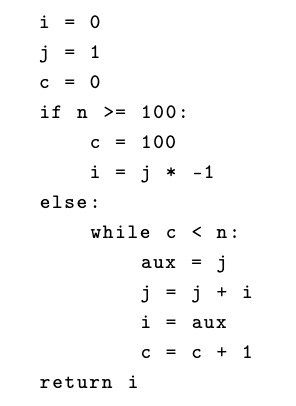
\includegraphics[width=0.3\textwidth]{Imagens/codigo-ex.jpg}
    \caption{Se $n >= 100$ retorna -1, senão retorna o n-ésimo número de Fibonacci}
    \label{fig:ex-codigo}
    \small{Fonte: O autor}
\end{figure}

% \begin{figure}[htpb]
% \lstset{%
%     caption=Exemplo de código que calcula o primeiro número de fibonatti maior que n,
%     basicstyle=\ttfamily\footnotesize\bfseries,
%     xleftmargin=.35\textwidth,
% }\label{list:ex-codigo}
% \begin{lstlisting}[language=Python]
% i = 0
% j = 1
% c = 0
% if n >= 100:
%     c = 100
%     i = j * -1
% else:
%     while c < n:
%         aux = j
%         j = j + i
%         i = aux
%         c = c + 1
% return i
% \end{lstlisting}
% \end{figure}

Na Figura \ref{fig:cfg-example1} é apresentado um exemplo de representação intermediária na forma de um Grafo de Fluxo de Controle referente ao código que calcula o número de Fibonacci presente da Figura \ref{fig:ex-codigo}. Nessa IR o código é representado por um grafo no qual cada nó contém um bloco de expressões sequenciais e novos nós e arestas são adicionados quando existem condicionais ou \emph{gotos} (vá para), expressando os diferentes caminhos possíveis de execução por meio de um grafo. Nessa representação intermediária os caminhos de execução no fluxos de controle do programa são evidenciados.

\begin{figure}
    \centering
    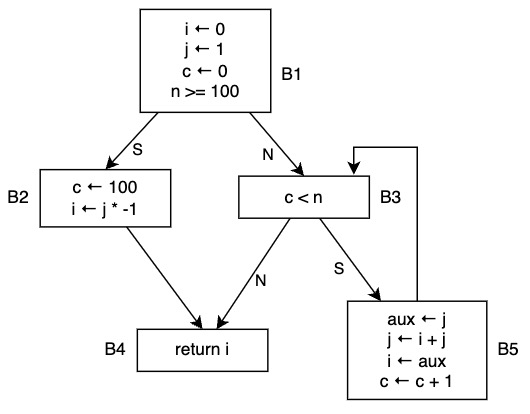
\includegraphics[width=0.6\textwidth]{Imagens/cfg-ex5.jpg}
    \caption{Exemplo de Grafo de IR em Fluxo de Controle da Figura \ref{fig:ex-codigo}}
    \label{fig:cfg-example1}
    \small{Fonte: O autor}
\end{figure}

Ao demonstrar os usos das IRs durante o processo de tradução de código, \citeonline{dragao} classifica-as em duas categorias, de acordo com seu uso ao longo da transformação do código fonte para código de máquina:

\begin{itemize}
\item \textbf{Representações Intermediárias de Alto Nível}: Estão mais próximas da linguagem fonte e são utilizadas nas primeiras etapas da tradução do código. Exemplos incluem as árvores sintáticas abstratas, que descrevem a estrutura direta do código fonte e são úteis em tarefas como a checagem estática de tipos.
\item \textbf{Representações Intermediárias de Baixo Nível}: Aproximam-se mais da máquina alvo e aparecem em etapas posteriores da tradução do código fonte. Focam em tarefas específicas da máquina alvo, como alocação de registradores e seleção de instruções.
\end{itemize}

Além dos usos já citados, com o advento das novas propostas de projeto de compiladores modulares e reutilizáveis, as IRs têm desempenhado um papel importante ao permitir a comunicação do \emph{frontend}, que é encarregado de fazer a leitura e tratamentos do código fonte, com o \emph{backend} que, por sua vez, faz otimizações, análises e pode gerar como saída o código de máquina para a arquitetura alvo. Nesse caso de uso a IR serve como uma linguagem para a comunicação entre as interfaces dos diferentes componentes do compilador \cite{lattner2004llvm}. 

A Figura \ref{fig:llvm-ri-ex1} apresenta um exemplo de IR especificada e usada pela LLVM, código que imprime no terminal a frase "Hello World!". Neste exemplo é possível observar que a representação intermediária gerada contém, além das definições e expressões necessárias, algum metadado que possivelmente será útil para as etapas seguintes da compilação. Na Seção \ref{sec:llvm-ir} a LLVM-IR será detalhada com mais profundidade.

\begin{figure}
    \centering
    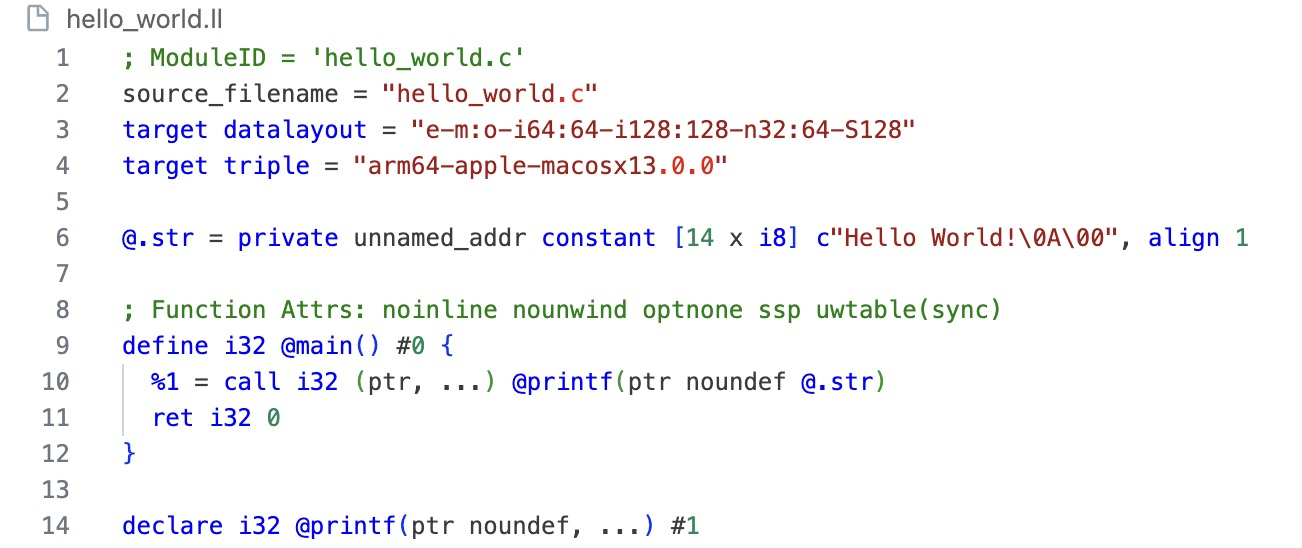
\includegraphics[width=0.8\textwidth]{Imagens/llvm-ir-ex1.jpg}
    \caption{Exemplo de IR em LLVM-IR}
    \label{fig:llvm-ri-ex1}
    \small{Fonte: O autor, gerado através do \emph{clang}}
\end{figure}

Ademais, é importante pontuar que, como visto nos exemplos, IRs podem ser tanto estruturas de dados armazenadas durante a execução do compilador, quanto uma linguagem em si, e seu uso vai depender de como o compilador foi projetado \cite{dragao}. Há inclusive a possibilidade de usar uma linguagem de programação como IR, por exemplo C, que compila para código nativo eficiente.

\section{Forma de Atribuição Única Estática}

É vastamente referenciado na literatura que a forma de atribuição única estática (SSA - \emph{Static Single-Assignment}) é de importante valor ao facilitar certas otimizações de código para linguagens imperativas \cite{appel1998ssa} \cite{dragao} \cite{muchnick1997advanced}. Sendo assim, utilizada de maneira ampla na implementação das etapas de otimização de código de compiladores e ferramentas de otimização de código, como é o caso da LLVM e do GCC (GNU Compiler Collection). % \cite{lattner2004llvm} https://pastel.hal.science/pastel-00002281/

Mais especificamente, \citeonline{muchnick1997advanced} traz alguns exemplos de algoritmos de otimização que SSA facilita e torna mais eficazes, principalmente referentes à análise do fluxo de dados de programas, como: propagação de constantes, numeração de valores, movimentação e remoção código invariante e remoção de redundância parcial. Segundo \citeonline{muchnick1997advanced}, isso segue do fato que na forma SSA há a separação dos valores contidos no programa, com base no lugar em que estes são usados.

Um procedimento está em forma de atribuição única estática quando cada variável que recebe um valor dentro dele é alvo de apenas uma atribuição \cite{muchnick1997advanced}. Ao passo que a cada atribuição uma nova variável deve ser criada, e dessa forma, as variáveis são imutáveis. Além disso, é definida a notação conceitual da função $\phi$, usada para unir definições de variáveis em caminhos divergentes no fluxo de controle, selecionando aquela pela qual o fluxo de controle passou durante a execução \cite{dragao}. Nota-se que a atribuição de uma variável pode ocorrer dentro de um laço de repetição, o que levaria a múltiplas definições desta, e iria contrariar as restrições da forma SSA. No entanto, a forma de atribuição única em SSA é uma característica estática do programa, e não uma propriedade dinâmica da execução \cite{appel1998ssa}. A Figura \ref{fig:not-ssa-vs-ssa} contém um exemplo de código e sua representação e ao lado sua representação em forma SSA, demonstrando a criação de novas variáveis a cada atribuição feita.

\begin{figure}[h]
\centering
\begin{subfigure}{.5\textwidth}
    \centering
    $$\displaylines{
    p \ \leftarrow \ a \ + \ b \cr
    q \ \leftarrow \ p \ - \ c \cr
    p \ \leftarrow \ p \ * \ q \cr
    p \ \leftarrow \ d \ - \ p \cr
    q \ \leftarrow \ p \ + \ q \cr
    }$$
    \caption{Não SSA}
    \label{fig:sub1}
\end{subfigure}%
\begin{subfigure}{.5\textwidth}
    \centering
    $$\displaylines{
    p_1 \ \leftarrow \ a \ + \ b \cr
    q_1 \ \leftarrow \ p_1 \ - \ c \cr
    p_2 \ \leftarrow \ p_1 \ * \ q_1 \cr
    p_3 \ \leftarrow \ d \ - \ p_2 \cr
    q_2 \ \leftarrow \ p_3 \ + \ q_1 \cr
    }$$
    \caption{Em forma SSA}
    \label{fig:sub2}
\end{subfigure}
\caption{Comparação entre atribuições em não SSA e em SSA}
\label{fig:not-ssa-vs-ssa}
\small{Fonte: O autor, adaptado de \citeonline{dragao}}
\end{figure}

O mecanismo padrão de tradução para a forma SSA é adicionar uma subscrição a cada variável toda vez que há uma atribuição, vide Figura \ref{fig:not-ssa-vs-ssa}, onde $p$ é dividido em $p_1$, $p_2$ e $p_3$ e $q$ se torna as duas variáveis $q_1$ e $q_2$. Porém, quando há mais de um caminho de execução em que uma mesma variável pode ser definida, há a necessidade de uma forma de unir estas. E é nesse momento que se faz o uso da função $\phi$, que tem a capacidade unir as definições divergentes de uma mesma variável nos pontos de junção do fluxo de controle.

A Figura \ref{fig:cfg-ssa-ex} contém um exemplo de como o programa da Figura \ref{fig:cfg-example1} fica na forma SSA. Nota-se o uso da função $\phi$ no ponto de junção para a variável $i$, o valor de $i_2$ naquele nó será atribuído ao valor do qual o fluxo de execução chega naquele bloco, podendo ter sido definida em B1 (onde é iniciado em 0) ou em B5 (recebendo o valor de aux$_1$).

\begin{figure}[h]
    \centering
    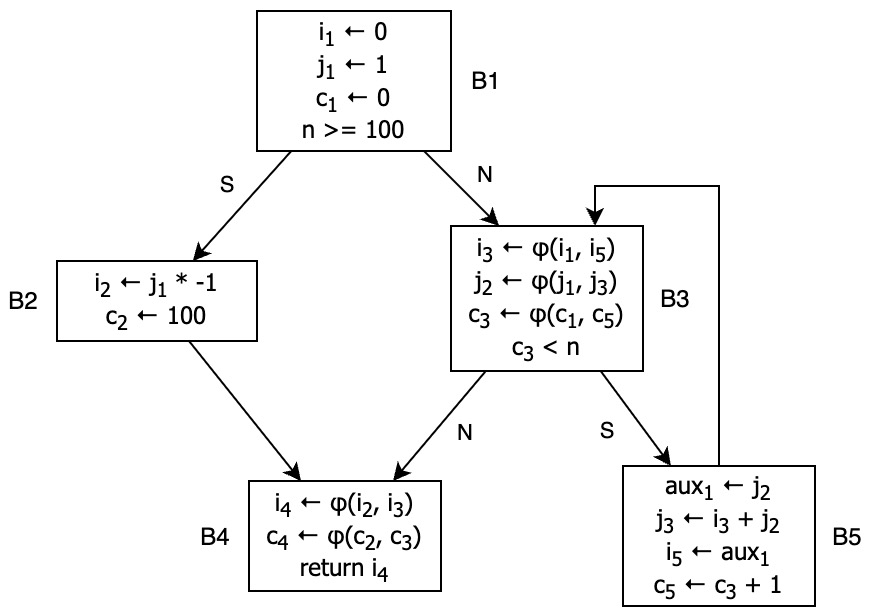
\includegraphics[width=0.6\textwidth]{Imagens/ssa-cfg-ex.jpg}
    \caption{CFG da Figura \ref{fig:cfg-example1} em forma SSA}
    \label{fig:cfg-ssa-ex}
    \small{Fonte: O autor}
\end{figure}

Há ainda o conceito de forma SSA mínima, que é a forma SSA que usa o menor número de funções $\phi$ possível. Para traduzir um código para a forma SSA mínima usa-se o conceito de fronteira de dominância (Definição \ref{def:dominance-frontier}) 
 \cite{cytron1991efficiently}.

É importante mencionar o uso de SSA na LLVM, um caso que demonstra a utilidade prática aplicada ao conjunto de ferramentas de compilação que está no estado da arte atualmente. Segundo \citeonline{lattner2004llvm}, a LLVM usa SSA como sua representação de código primária (exceto para definições de locação de memória), em que cada registrador virtual é escrito à exatamente uma instrução, e cada uso de registrador é dominado (Definição \ref{def:domination}) pela sua definição. \citeonline{lattner2004llvm} defendem o uso da forma SSA dizendo que esta oferece uma representação simplificada do fluxo de dados, facilitando muitas otimizações e possibilitando que algoritmos mais rápidos que não dependem do fluxo (\emph{flow-insensitive}) tirem proveito das vantagens de algoritmos que são sensíveis ao fluxo (\emph{flow-sensitive}), sem o custo de análises complexas no fluxo de dados. Adicionalmente, as mudanças que não envolvem \emph{loops} nessa estrutura são mais simples, já que não se deparam com dependências contrárias ou de saída em suas variáveis \cite{lattner2004llvm}.

\subsection{Árvore de Dominância} \label{sub:arvore-dominancia}

Conceitos advindos da teoria dos grafos como: dominância, fronteira de dominância, dominância imediata e árvore de dominância, são essenciais para este trabalho e são utilizados inclusive no método de tradução descrito no Capítulo \ref{cap:desenvolvimento}.

\begin{definition}[Dominação]\label{def:domination}
Na teoria de grafos, mais especificamente em grafos de fluxo, um nó $d$ é dito dominar um nó $n$ se, a partir do nó inicial, todos os caminhos até $n$ devem passar pelo nó $d$ \cite{muchnick1997advanced}. Notacionalmente $d \
dom \ n$. Nota-se que, por definição, todos os nós dominam si mesmos.
\end{definition}

\begin{definition}[Dominação Estrita]
Em um grafo de fluxo, um nó $d$ domina estritamente um nó $n$ se $d$ domina $n$ e $d \neq n$. Notacionalmente $d \ sdom \ n$.
\end{definition}

\begin{definition}[Predecessor e Predecessor Imediato]
Em um grafo de fluxo, um nó $n$ é predecessor de $m$ ($n \ pred \ m$) se existe pelo menos um caminho da origem até $m$ que passa por $n$; $n$ é considerado predecessor imediato ($Pred$) se em algum caminho é utilizada uma aresta de $m$ para $n$.
\end{definition}

\begin{definition}[Dominância Imediata]
O dominador imediato de um nó $n$ é o único nó que, domina estritamente $n$, mas não domina nenhum outro nó que domina estritamente $n$. Observa-se que todos os nós em um grafo de fluxo tem um dominador imediato, com exceção do inicial.
\end{definition}

\begin{definition}[Fronteira de Dominância]\label{def:dominance-frontier}
Sendo $x$ um nó do grafo de fluxo de controle, a fronteira de dominância de $x$ é o conjunto de todos os nós $y$ no grafo de fluxo tal que $x$ domina um predecessor imediato de $y$, mas não domina estritamente $y$ \cite{cytron1991efficiently}.
\end{definition}

Esses conceitos são principalmente utilizados ao analisar a dominância e dependência dos blocos dentro do grafo de fluxo de controle. Percebe-se que, se um bloco do grafo de fluxo de controle $n$ é dominado por outro nó $d$, as variáveis do bloco $d$ existem e podem ser acessadas no bloco $n$. Com isso, a estrutura de árvore de dominância favorece essa análise ao fornecer informação sobre o escopo das variáveis de um procedimento.

\begin{definition}[Árvore de Dominância]\label{def:dom-tree}
A árvore de dominância de um dado grafo de fluxo é a árvore em que os filhos de cada nó $n_i$ são os nós dominados imediatamente por $n_i$. A raiz da árvore é o nó inicial.
\end{definition}

A Figura \ref{fig:dominance-ex} contém um exemplo de árvore de dominância lado a lado ao grafo de fluxo de controle do código de exemplo da Figura \ref{fig:cfg-example1}. Percebe-se que o nó B4 é dominado somente pelo bloco B1 uma vez que há caminhos da origem até B4 que passam por B2 ou B3.

\begin{figure}
\centering
\begin{subfigure}{.5\textwidth}
  \centering
  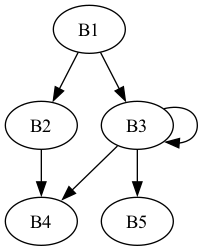
\includegraphics[width=.5\linewidth]{Imagens/graph-fig2.png}
  \caption{Grafo de fluxo de controle}
  \label{fig:sub1}
\end{subfigure}%
\begin{subfigure}{.5\textwidth}
  \centering
  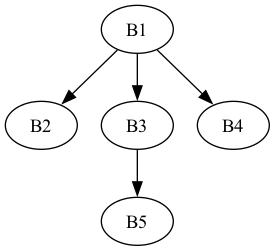
\includegraphics[width=.6\linewidth]{Imagens/dominance-fig2.png}
  \caption{Árvore de dominância}
  \label{fig:dom-tree}
\end{subfigure}
\caption{Comparação entre CFG e Árvore de Dominância do Código da Figura \ref{fig:cfg-example1}}
\label{fig:dominance-ex}
\small{Fonte: O autor}
\end{figure}

\section{ANF}

A Forma A-normal (ANF) é um conceito importante na compilação de programas funcionais, sendo utilizado frequentemente para simplificar a estrutura dos programas e facilitar otimizações. \citeonline{sabry1992reasoning} introduziram ANF como uma alternativa mais simples ao estilo de passagem de continuações (CPS, do inglês \emph{Continuation Passing Style}), demonstrando sua efetividade em transformações e otimizações de código funcional.

% \begin{figure}[h]
% \begin{center}
% \large
% \begin{tabular}{r@{\ \ }c@{\ \ }l}
%     $e$ & ::= & $v$ \ $|$ \ $e \ e$ \ $|$ \ $\lambda x. e$ \\
%     $v$ & ::= & $x$ \ $|$ \ $c$ \\
%     $x$ & $\in$ & \emph{variáveis} \\
%     $c$ & $\in$ & \emph{constantes} \\
% \end{tabular}
% \caption{Gramática Cálculo Lambda}
% \small{Fonte: O autor}
% \end{center}
% \label{fig:calculo-lambda}
% \end{figure}

% \igor{próximo parágrafo ta WIP}

% Em cálculo lambda puro, expressões podem ser: um valor, uma aplicação, ou uma abstração $\lambda$, vide a Figura \ref{fig:calculo-lambda}. Variáveis que não estão vinculadas a uma abstração $\lambda$ são ditas variáveis livres, o conjunto das variáveis livres de um termo $M$ é $FV(M)$. Em calculo lambda, é possível obter expressões como: $f \ (g \ 2) \ (h \ 3)$. Ao buscar por regras de redução para programas funcionais que pudessem prover um conjunto de axiomas no qual é possível provar que para dois termos $M$ e $N$, se $M = N$ então $CPS(M) = CPS(N)$. \citeonline{sabry1992reasoning} formularam as reduções vistas na Figura \ref{fig:reducoes} sobre a representação intermediária CPS. Após ter formulado tais regras, \citeonline{flanagan1993essence} descobrem o cálculo $\lambda_{\, v} \, A$, que não permite que tais reduções possam ser feitas, ou seja, o programa já está otimizado para as regras $\beta_{lift}$ e $\beta_{flat}$.

% \begin{figure}[h]
% \centering
% \begin{align*}
% ((\lambda x.M) \ V) & \rightarrow M[x := V] & & & & (\beta_v) \\
% (\lambda x.V x) & \rightarrow V & & x \notin FV(V) & & (\eta_v) \\
% E[((\lambda x.M) \ N)] & \rightarrow ((\lambda x.E[M]) \ N) & & x \notin FV(E) & & (\beta_{lift}) \\
% E[((M \ N) \ L)] & \rightarrow ((\lambda x.E[(x \ L)]) (M \ N)) & & x \notin FV(E, L) & & (\beta_{flat}) \\
% ((\lambda x.x) \ M) & \rightarrow M & & & & (\beta_d) \\
% ((\lambda x.E[(y \ x)]) \ M) & \rightarrow E[(y \ M)] & & x \notin FV(E[y]) & & (\beta_{\Omega})
% \end{align*}
% \caption{Reduções $A$ em CPS: $\{\eta_v, \beta_v, \beta_{lift}, \beta_{flat}, \beta_d, \beta_{\Omega}\}$}
% \label{fig:reducoes}
% \small{Fonte: \citeonline{sabry1992reasoning}}
% \end{figure}

Fundamentalmente, ANF é uma restrição a termos do cálculo-$\lambda$, na qual é imposto que os termos lambda sejam escritos em estilo direto \cite{ssaToAnf}. Em suma, isso quer dizer que os argumentos em aplicações de expressões devem ser termos atômicos (variáveis ou constantes). E que, para haver continuações na computação, são usadas variáveis temporárias atribuídas às sub-expressões do procedimento, e que são definidas em expressões \emph{let}. A Figura \ref{fig:llvm-ir-gramatica} apresenta um exemplo de gramática livre de contexto na qual não há como aninhar aplicações de expressões, sendo necessário que uma aplicação seja atribuída a uma variável antes de ser utilizada, ou seja, uma gramática na qual as produções são na forma ANF. Na notação utilizada, as classes gramaticais indicadas por uma linha superior (\emph{overline}) representam sequências de zero ou mais ocorrências dessas produções gramaticais. Pontua-se que ANF é definido conforme o cálculo-$\lambda$ com avaliação \emph{call-by-value} definido por \citeonline{plotkin1975call}.

\begin{figure}[h]
\begin{center}
\large
\begin{tabular}{r@{\ \ }c@{\ \ }l}
    $e$ & ::= & \textbf{let} \ $x$ \ \textbf{=} \ $v \ \overline{v}$ \ \textbf{in} \ $e$ \\
    & \ \ $|$ & $v \ \overline{v}$ \\
    $v$ & ::= & $x$ \ $|$ \ $c$ \ $|$ \ $\lambda x . e$ \\
    $x$ & $\in$ & \emph{variáveis} \\
    $c$ & $\in$ & \emph{constantes} \\
\end{tabular}
\caption{Gramática Exemplo de ANF}
\label{fig:llvm-ir-gramatica}
\small{Fonte: O autor}
\end{center}
\end{figure}

Em ANF o grafo de fluxo de controle é explícito, uma vez que chamadas de cauda são claramente distinguidas por sua posição dentro das expressões \emph{let}: chamadas de função no lado direito de uma atribuição de variável indicam chamadas normais, enquanto aquelas que aparecem no corpo significam chamadas de cauda, ou \emph{jumps} no fluxo de controle \cite{ssaToAnf}. Essa representação explícita de chamadas e chamadas de cauda simplifica análises sobre a execução do programa e facilita as otimizações nesse sentido. A Figura \ref{fig:lambda-vs-anf} apresenta um exemplo de como uma expressão fica quando escrita em ANF.

Semelhante à forma SSA, ANF codifica explicitamente o fluxo de dados ao nomear todas as sub-expressões dentro do programa e ao permitir apenas uma definição para cada variável \cite{ssaToAnf}. No entanto, ANF impõe essa restrição dinamicamente, pois um novo escopo é criado em tempo de execução para cada invocação de função. O escopo sintático claro em ANF facilita muitas otimizações que envolvem movimento de código entre blocos, o que pode ser mais complexo em SSA devido à necessidade de manter a propriedade de dominância entre a definição e uso das variáveis \cite{ssaToAnf}.

\begin{figure}[h]
\centering
\begin{subfigure}{.5\textwidth}
    \centering
    \begin{lstlisting}[language=Haskell,xleftmargin=.1\textwidth]
h (f (g x + 1)) (k (y * 2))
    \end{lstlisting}
    \caption{Não ANF}
    \label{fig:sub1}
\end{subfigure}%
\begin{subfigure}{.5\textwidth}
    \centering
    \begin{lstlisting}[language=Haskell,xleftmargin=.2\textwidth]
let a = g x in
let b = a + 1 in
let c = y * 2 in
let d = k c in
let e = f b in
h e d
    \end{lstlisting}
    \caption{Em ANF}
    \label{fig:sub2}
\end{subfigure}
\caption{Comparação de uma expressão em ANF}
\label{fig:lambda-vs-anf}
\small{Fonte: O autor}
\end{figure}

Dadas suas vantagens e aplicabilidade no paradigma funcional, variantes de ANF são usadas na prática como representação intermediária de diversos compiladores de linguagens funcionais, como GHC de Haskell \cite{jones1998transformation}, e TIL de ML \cite{wegman1991constant}. Ao usar ANF, estas ferramentas acrescentam algumas características como: permitir tuplas, funções com mais de um argumento, operações primitivas e condicionais. Na Seção \ref{sec:desenvolvimento-anf} é apresentada a gramática livre de contexto variante de ANF desenvolvida neste trabalho, e que é a saída do método de tradução desenvolvido.

\subsection{Tradução entre SSA e ANF}

Devido às características em comum de, por exemplo, não permitir mais de uma atribuição a uma mesma variável e ter o fluxo de controle explícito, pode-se inferir que existe uma relação entre a forma SSA e programação funcional. Mais do que isto, \citeonline{kelsey1995correspondence} e \citeonline{appel1998ssa} demonstraram que ambas são correspondentes, existindo um algoritmo que faz a tradução estática entre elas.

De maneira mais formal, \citeonline{ssaToAnf} definem um procedimento para a tradução de SSA para ANF, e demonstram que uma otimização, que é geralmente feita através de SSA, também pode ser feita utilizando ANF. O procedimento de \citeonline{ssaToAnf} servirá como base para a implementação deste trabalho apresentada no Capítulo \ref{cap:desenvolvimento}. Fazer a tradução de SSA para ANF envolve a construção da árvore de dominância (vista na Seção \ref{sub:arvore-dominancia}) sobre o grafo de fluxo de controle da forma SSA. A árvore serve como base para a construção dos escopos das funções em ANF. No código em ANF as funções correspondem tanto ao programa completo, quanto a estrutura do grafo de fluxo de controle de um procedimento específico \cite{ssaToAnf}. Os parâmetros das funções são determinados pelos $\phi$s do bloco de SSA, e o \emph{jumps} são traduzidos para chamadas de cauda.

\begin{figure}[h]
    \centering
\lstset{%
    xleftmargin=.17\textwidth,
}    
\begin{lstlisting}[language=Haskell,style=nasm]
fib n =
  let b1 () =
        let i1 = 0
            j1 = 1
            c1 = 0
            b2 () =
              let c2 = 100
                  i2 = j1 * (-1)
              in b4 i2 c2
            b3 i3 j2 c3 =
              let b5 () =
                    let aux1 = j2
                        j3 = i3 + j2
                        i5 = aux1
                        c5 = c3 + 1
                    in b3 i5 j3 c5
              in if c3 < n then b5 ()
                           else b4 i3 c3
            b4 i4 c4 = let in i4
        in if n >= 100 then b2 ()
                       else b3 i1 j1 c1          
    in b1 ()
\end{lstlisting}    
    \caption{Programa funcional em ANF em Haskell referente ao CFG da Figura \ref{fig:cfg-ssa-ex}}
    \label{fig:eq-ssa-func}
    \small{Fonte: O autor}
\end{figure}

A Figura \ref{fig:eq-ssa-func} contém um exemplo de código em ANF referente ao SSA da Figura \ref{fig:cfg-ssa-ex}. Nessa sintaxe, o ANF desse código é executável no GHC. Observa-se nesse exemplo que cada bloco é traduzido para uma função. Dentro do escopo dos blocos estão também as funções referentes aos blocos imediatamente dominados por estes. Os $\phi$s do bloco determinam seus argumentos, e para determinar o valor dos argumentos nas chamadas de função é necessário buscar o valor que seria atribuído pelo $\phi$ a partir do bloco que está fazendo a chamada.

No que se refere a este trabalho, \citeonline{rigon2020inferring} exploraram tal correspondência ao propor a definição do núcleo de uma linguagem puramente funcional, e a implementação de um algoritmo de inferência de tipos para código funcional que é gerado a partir de sua representação em forma SSA.

\section{LLVM}

O \emph{framework} LLVM (do inglês Máquina Virtual de Baixo Nível) foi projetado e desenvolvido com a proposta de oferecer um conjunto de ferramentas para análise e transformação de código arbitrário \cite{lattner2004llvm}. Este \emph{framework} vem se consolidando desde sua criação, e tornou-se uma parte fundamental no design de diversos compiladores modernos, sendo adotado por grandes empresas de tecnologia como Apple com o \emph{clang}, Google na plataforma Android e Mozilla com Rust. Isso se deve principalmente devido à sua capacidade de otimização de código, suporte a várias linguagens de programação e designs de hardware, e arquitetura modular que favorece o acoplamento de seus módulos em outros sistemas.

Segundo \citeonline{lattner2004llvm}, a LLVM tem dois principais pontos que a diferenciam das demais soluções, e que serão melhor explorados nessa seção: o projeto do compilador e a representação intermediária utilizada no \emph{framework}. Segundo \citeonline{lattner2004llvm}, o compilador é construído num modelo modular que é capaz de explorar a LLVM-IR como interface desses módulos, dessa forma fornecendo uma vasta combinação de capacidades quanto à otimização e tradução de código.

A Figura \ref{fig:llvm-design} apresenta uma visão de alto nível da arquitetura do sistema da LLVM e é explicada pelos autores como segue:

\begin{citacao}
Resumidamente, compiladores \emph{frontend} estáticos emitem código na representação da LLVM, que será então combinado pelo LLVM linker. O linker faz uma série de otimizações em \emph{link-time}, especialmente as inter-procedurais. O código LLVM resultante é traduzido para código nativo para uma dada arquitetura alvo em \emph{link-time} ou \emph{install-time}, e o código LLVM é então salvo em código nativo (é possível traduzir o código LLVM em tempo de execução, com um tradutor \emph{just-in-time}). O gerador de código nativo insere uma instrumentação leve para identificar partes do código frequentemente executadas e que podem ser otimizadas em tempo de execução. Os dados de perfil coletados em tempo de execução representam as execuções do usuário final (não do desenvolvedor) e podem ser usados por um otimizador \emph{offline} para realizar otimizações agressivas diretamente orientadas por perfil durante o tempo ocioso, adaptadas à máquina alvo específica. \cite{lattner2004llvm}
\end{citacao}

\begin{figure}[H]
    \centering
    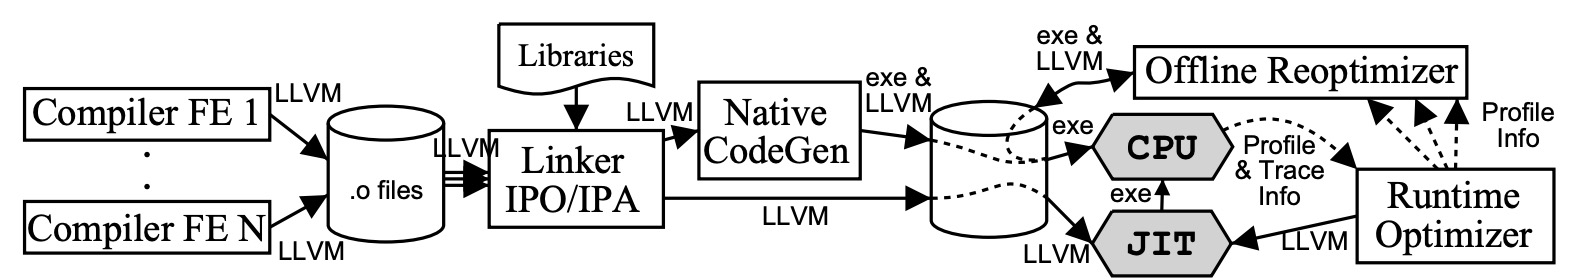
\includegraphics[width=\textwidth]{Imagens/llvm-design.jpg}
    \caption{Diagrama da arquitetura do sistema da LLVM}
    \small{Fonte: \citeonline{lattner2004llvm}}
    \label{fig:llvm-design}
\end{figure}

\citeonline{lattner2004llvm} também argumentam que a arquitetura projetada para a LLVM provê estas cinco capacidades que, em conjunto, a diferencia das demais soluções: (1) modelo de compilação contínua, (2) geração de código \emph{offline}, (3) perfilagem (\emph{profilling}) e otimizações baseadas no usuário, (4) modelo de \emph{runtime} transparente, e (5) compilação uniforme de todo o programa. 

% Compiladores tradicionais oferecem geração de código offline e modelo de tempo de execução transparente, mas carecem de compilação contínua, perfilagem baseada no usuário e compilação de todo o programa. Alguns compiladores comerciais exportam representações intermediárias para otimização em \emph{link-time}, mas não suportam otimização em tempo de execução ou \emph{offline}. Máquinas virtuais de alto nível, como a JVM (Java Virtual Machine), fornecem perfilagem baseada no usuário e compilação contínua parcial, mas faltam geração de código \emph{offline} e modelo de \emph{runtime} transparente. Otimizadores de tempo de execução binário transparentes, como o Dynamo, oferecem geração de código \emph{offline}, modelo de tempo de execução transparente e compilação de todo o programa, mas são limitados na capacidade de otimização devido ao foco em código binário nativo. A Otimização Guiada por Perfil (PGO) para linguagens estáticas oferece perfilagem baseada no usuário, mas não é transparente e pode levar a desempenho sub-ótimo se o treinamento não refletir os padrões de uso reais.

Conforme anteriormente citado, a parte que fundamenta e integra todos os módulos e funcionalidades da LLVM é a sua representação intermediária, a LLVM-IR, que será melhor detalhada na próxima seção.

\subsection{LLVM-IR}\label{sec:llvm-ir}

A representação intermediária de código definida pela LLVM (fundamentada no modelo SSA), traz algumas funcionalidades inovadoras, e serve como uma forma unificada de representar código para fins de análise, modificação e distribuição durante todo o processo de transformação de código \cite{lattner2004llvm}. A especificação de tal representação consiste em um conjunto de instruções similares a de um processador do tipo RISC (do inglês, \emph{Reduced Instruction Set Computer}), mas com informações de alto nível importantes para análises eficazes do código a ser gerado. \citeonline{lattner2004llvm} colocam três principais aspectos:

\begin{enumerate}
    \item[(a)] Um sistema de tipos de baixo nível que pode ser usado para implementar tipos de dados e operações das linguagens de alto nível, expondo os comportamentos implementados a todas as etapas de otimização. Este sistema de tipos inclui informações de tipo que poderão ser usadas por técnicas sofisticadas (independentes de linguagem), como algoritmos para análise de ponteiros, análise de dependências e transformações de dados.
    \item[(b)] Instruções para fazer conversão dos tipos e aritmética de endereços de baixo nível, preservando a informação de tipagem.
    \item[(c)] Duas instruções para tratamento de exceções em baixo nível para implementação de semânticas de exceção específicas das linguagens, mantendo explícito o fluxo de controle ao compilador. 
\end{enumerate}

Quanto à estrutura do código, na representação intermediária da LLVM o fluxo de controle fica explícito, uma vez que "uma função é um conjunto de blocos básicos, e cada bloco básico é uma sequência de instruções LLVM, terminando em exatamente uma instrução terminadora [...]. Cada terminador especifica explicitamente seus blocos básicos sucessores." \cite{lattner2004llvm}.

Segundo a referência da linguagem, o conjunto de instruções da LLVM-IR conta atualmente com mais de 60 códigos de operação (\emph{opcodes}). Dentre estas estão instruções de operações matemáticas, operações em ponteiros, operadores de comparação, instruções de terminação (\emph{return}, \emph{branch}), e também operações mais específicas da solução da LLVM, como conversão entre tipos com diversas opções. O sistema de tipos da LLVM permite a sobrecarga dos operadores para mais de um tipo, ou seja, a instrução \emph{add} por exemplo pode ser usada tanto para inteiros de qualquer tamanho, quanto para ponto flutuantes \cite{llvmLangRef}.

Uma funcionalidade importante do sistema da LLVM, apesar de não visada diretamente nesse trabalho, é o sistema de tipos da LLVM-IR, que conta com diversos tipos nativos, uma robusta instrumentação para definição de tipos compostos, e que é independente da linguagem fonte. Na LLVM todas as variáveis e objetos na memória da representação SSA têm um tipo associado, e todas as operações devem se submeter a regras de tipo específicas \cite{lattner2004llvm}. O sistema de tipos compreende tipos como: \emph{void}, booleano, inteiros com ou sem sinal de 8 até 64 bits e ponto flutuante de precisão simples ou dupla. Além disso, a LLVM contém somente 4 tipos derivados: ponteiros, arrays, estruturas e funções \cite{llvmLangRef}.

A seguir há um código em LLVM-IR gerado utilizando o compilador \emph{clang} a partir de um código em C++. O clang foi utilizado pois a ferramenta de linha de comando tem uma opção para emitir código em LLVM-IR. A versão do \emph{clang} utilizada foi a 15.0.0 em um notebook com processador \emph{Apple M1 Pro}. O comando exato para emitir esse código foi: \verb|clang -emit-llvm -S -O1 fact.cpp|, as flags \verb|-emit-llvm -S| servem para que o \emph{clang} dê como saída código em LLVM-IR e a flag \verb|-O1| foi utilizada por dar a saída já com algumas otimizações e já em forma SSA.

\begin{figure}[h]
    \centering
\begin{lstlisting}[language=llvm,style=nasm]
; ModuleID = 'myfib.c'
source_filename = "myfib.c"
target datalayout = "e-m:o-i64:64-i128:128-n32:64-S128"
target triple = "arm64-apple-macosx14.0.0"

; Function Attrs: nofree norecurse nosync nounwind readnone ssp uwtable(sync)
define i32 @fib(i32 noundef %0) local_unnamed_addr #0 {
  %2 = icmp sgt i32 %0, 99
  br i1 %2, label %12, label %3

3:                                                ; preds = %1
  %4 = icmp sgt i32 %0, 0
  br i1 %4, label %5, label %12

5:                                                ; preds = %3, %5
  %6 = phi i32 [ %8, %5 ], [ 0, %3 ]
  %7 = phi i32 [ %10, %5 ], [ 0, %3 ]
  %8 = phi i32 [ %9, %5 ], [ 1, %3 ]
  %9 = add nsw i32 %6, %8
  %10 = add nuw nsw i32 %7, 1
  %11 = icmp eq i32 %10, %0
  br i1 %11, label %12, label %5, !llvm.loop !6

12:                                               ; preds = %5, %3, %1
  %13 = phi i32 [ -1, %1 ], [ 0, %3 ], [ %8, %5 ]
  ret i32 %13
}

attributes #0 = { nofree norecurse nosync nounwind readnone } ; ...

!llvm.module.flags = !{!0, !1, !2, !3, !4}
!llvm.ident = !{!5}

!0 = !{i32 2, !"SDK Version", [2 x i32] [i32 14, i32 4]}
!1 = !{i32 1, !"wchar_size", i32 4}
; ... continua com mais metadados
\end{lstlisting}                                         
    \caption{Exemplo de Código em LLVM-IR}
    \label{fig:exemplo-llvm-ir}
    \small{Fonte: O autor, gerado usando \emph{clang} e editado}
\end{figure}

Trazendo uma visão geral sobre o código da Figura \ref{fig:exemplo-llvm-ir}: no começo do código há metadados quanto ao arquivo de origem e à arquitetura alvo; linhas iniciadas em ";"\ são comentários; na definição da função, além dos tipos que são obrigatórios, há algumas \emph{flags} para otimização; dentro dos colchetes estão os blocos da forma SSA, o primeiro bloco não necessita explicitamente de um \emph{label}, mas recebe implicitamente o próximo registrador do SSA disponível (nesse caso o "\%1", já que o argumento usa o "\%0"). Também é interessante notar as operações \verb|phi| e \verb|br| (\emph{branch}) e seus argumentos e que todas as operações e instruções carregam tipagem explícita.

A LLVM-IR ser fundamentada na forma SSA quer dizer que cada registrador virtual (variável) é definido exatamente uma vez e o uso de um registrador deve ser dominado por sua definição \cite{lattner2004llvm}; e a LLVM-IR conta com a instrução \verb|phi| explícita, que corresponde diretamente à função $\phi$ da forma SSA \cite{lattner2004llvm}.


\chapter{Desenvolvimento}\label{cap:desenvolvimento}

Como referenciado, a correspondência entre SSA e programação funcional já foi explorada por vários trabalhos que buscaram entender como extrair valor deste fato. Notoriamente, \citeonline{rigon2020inferring} exploram esta correspondência ao propor o núcleo de uma linguagem pseudo-imperativa com sistema de tipo e efeitos baseados no trabalho de \citeonline{leijen2014koka} usando a forma SSA traduzida do código em Koka.

O presente trabalho implementa uma proposta de extensão do trabalho de \citeonline{rigon2020inferring}, agora traduzindo código genérico para programação funcional (em ANF), a partir da representação intermediária da LLVM. Levando a possibilidade de, no futuro, ser pesquisada a inferência de efeitos em código em LLVM-IR, consequentemente código gerado a partir de linguagens imperativas.

Uma das propostas de valor deste trabalho é apresentada na Figura \ref{fig:proposta}, demonstrando a possibilidade de tradução de código arbitrário para código funcional. A partir de código em alguma linguagem fonte como C, C++ ou Rust, a LLVM é utilizada para gerar a LLVM-IR em forma SSA. A representação intermediária gerada é então usada como entrada para o método proposto nesse trabalho, que faz a tradução da representação intermediária da LLVM para código funcional em forma ANF na linguagem Haskell. Porém, essa é ainda uma exploração inicial dessa tradução, já que nesse trabalho é interpretado somente um subconjunto da representação intermediária da LLVM.

\begin{figure}[h]
    \centering
    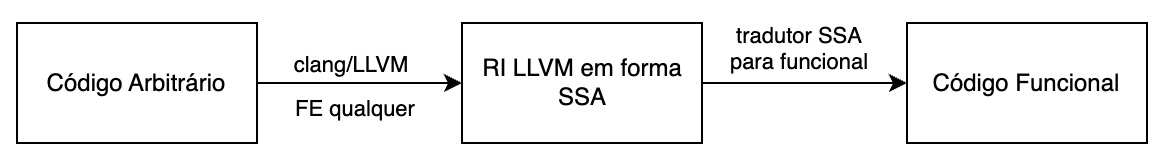
\includegraphics[width=\textwidth]{Imagens/proposta2.jpg}
    \caption{Diagrama da Proposta do Sistema de Tradução}\
    \label{fig:proposta}
    \small{Fonte: O autor}
\end{figure}

O método de tradução proposto neste trabalho foi implementado em duas fases: inicialmente criando um \emph{parser} (analisador sintático) para um subconjunto da representação intermediária da LLVM, e então desenvolvendo uma adaptação do método descrito por \citeonline{ssaToAnf} para traduzir a LLVM-IR em forma SSA para uma representação intermediária similar à ANF que é apresentada como código em linguagem Haskell. O objetivo da geração do código na sintaxe de Haskell é facilitar a validação do trabalho, uma vez que dessa forma programas que não apresentam efeitos colaterais poderão ser executados.

\section{\emph{Parser} da LLVM-IR}

A primeira etapa para a tradução é a implementação de um \emph{parser} da LLVM-IR para que, com base no código interpretado, a tradução seja aplicada. Deste modo, a gramática usada para a interpretação foi desenvolvida com base em exemplos gerados usando o \emph{clang} em código C++, e com base na documentação de referência da linguagem que é fornecida pela LLVM\footnote{https://llvm.org/docs/LangRef.html}.

Visto que a LLVM-IR conta com diversas funcionalidades de alto e baixo nível, no código podem ser geradas diversas informações como: metadados, informação para depuração, \emph{flags} de otimização, etc \cite{llvmLangRef}. Entre estas, há muitas operações, palavras reservadas e funções nativas que não são úteis ou fogem do escopo deste trabalho. Devido a isso e ao tempo disponível para desenvolvimento, um subconjunto da linguagem intermediária foi selecionado. Nesse subconjunto o escopo global só permite definição de funções, sem variáveis ou demais dados globais. Ademais, para simplificar o escopo deste trabalho, constantes foram limitadas somente a numerais de tipos inteiros de qualquer tamanho.

\begin{figure}[h]
\begin{center}
\large
\begin{tabular}{r@{\ \ }c@{\ \ }l}
    $p$ & ::= & $\textbf{define} \ t \ x \ \textbf{(} \ \overline{t \ \ x} \ \textbf{)}\ \textbf{\{}\ \overline{b}\ \textbf{\}}$ \\
    $b$ & ::= & $x$ \ \textbf{:} \ $\overline{\phi}$ \ $\overline{s}$ \ $f$ \\
    $\phi$ & ::= & $x$ \ \textbf{=} \ $\textbf{phi}$ \ $t$ \ $\overline{a}$ \\
    $s$ & ::= & $x$ \ $\boldsymbol{=}$ \ $o$ \ $|$ \ $x$ \ $\boldsymbol{=}$ \ $q$ \\
    $q$ & ::= & \textbf{call} \ $t$ \ $x$ \ $\textbf{(} \ \overline{t \ v} \ \textbf{)}$ \\
    $f$ & ::= & \textbf{br} \ $t$ \ $x$ \ $|$ \ \textbf{br} \ $t$ \ $v$ \ \textbf{,} \ $t$ \ $x$ \ \textbf{,} \ $t$ \ $x$ $|$ \ \textbf{ret} \ $t$ \ $v$ \\
    % $\overline{a}$ & ::= & $a$ \ \textbf{,} \ $\overline{a}$ \\
    % $\overline{x}$ & ::= & $t$ \ $x$ \ \textbf{,} \ $\overline{x}$ \ $|$ \ $t$ \ $x$ $|$ \ $\epsilon$\\
    $a$ & ::= & $\textbf{[}$ \ $v$ \ \textbf{,} \ $x$ \ \textbf{]} \\
    $o$ & ::= & $\beta$ \ $t$ \ $v$ \ \textbf{,} \ $v$ \ $|$ \\ 
    & & $\mathbf{icmp}$ \ $\tau$ \ $t$ \ $v$ \ \textbf{,} \ $v$ \ $|$ \\
    & & \textbf{select} \ $t$ \ $v$ \ \textbf{,} \ $t$ \ $v$ \ \textbf{,} \ $t$ \ $v$ \ $|$  \\ 
    & & $\mu$ \ $t$ \ $v$ \ \textbf{to} \ $t$ \\
    $v$ & ::= & $x$ $|$ $c$ \\
    $t$ & $\in$ & \emph{tipos nativos da LLVM}  \\
    $x$ & $\in$ & \emph{variáveis locais ou globais} \\
    $c$ & $\in$ & \emph{constantes} \\
    $\beta$ & $\in$ & \emph{operações binárias da LLVM} \\
    $\tau$ & $\in$ & \emph{opções de comparação da LLVM} \\
    $\mu$ & $\in$ & \emph{operações de conversão da LLVM} \\
\end{tabular}
\caption{Gramática de interpretação da LLVM-IR}
\label{fig:llvm-ir-gramatica}
\small{Fonte: O autor}
\end{center}
\end{figure}

Conforme a gramática presente na Figura \ref{fig:llvm-ir-gramatica}, os procedimentos em LLVM-IR tratados nesse trabalho são na seguinte forma: a definição de uma função se dá pelo seu tipo, nome, os seus parâmetros, e os blocos da forma SSA. Os blocos são definidos por seu \emph{label} e devem conter, nessa ordem, uma sequência de $\phi$s, em seguida as declarações de variáveis, e por último um \emph{jump} no fluxo de controle (por exemplo, retorno ou \emph{branch}). É determinado que todos os blocos e argumentos precisam ter um \emph{label}, ou seja, precisam ser nomeados. Nesta gramática o não terminal $o$ representa as operações nativas da LLVM, nas quais estão compreendidas operações matemáticas, de comparação, conversão, entre outras. Essas operações nativas foram mapeadas e traduzidas para operações correspondentes em linguagem Haskell, para que o código gerado possa ser executado. Na Seção \ref{cap:desenvolvimento-traducao} há mais detalhes sobre como essas operações foram traduzidas. Observa-se também que na LLVM-IR não há necessidade de um terminador de linha como ";" \ ou até mesmo uma nova linha para a próxima instrução. Devido a isso, a gramática não contém nenhum terminal pontuando o fim de uma linha.

A Figura \ref{fig:exemplo-entrada} apresenta um exemplo de código bem formatado que é gerado pela gramática definida. Neste exemplo foram removidas \emph{flags} de otimização, informação para depuração e outras informações que são ignoradas durante a análise léxica. Nota-se que os tipos fazem parte da estrutura do código na linguagem de entrada. Posteriormente esses tipos são desconsiderados ao gerar a representação ANF em código. Ao final desta etapa obtêm-se uma representação em memória do SSA interpretado, com toda a informação necessária para fazer a tradução descrita na Seção \ref{cap:desenvolvimento-traducao}.

\begin{figure}
\centering
\lstset{xleftmargin=.25\textwidth}
\begin{lstlisting}[language=llvm,style=nasm]
define i32 @factorial(i32 %0) {
1:
  br label %2

2:
  %3 = phi i32 [ 1, %1 ], [ %8, %6 ]
  %4 = phi i32 [ %0, %1 ], [ %7, %6 ]
  %5 = icmp slt i32 %4, 2
  br i1 %5, label %9, label %6

6:
  %7 = add nsw i32 %4, -1
  %8 = mul nsw i32 %3, %4
  br label %2

9:
  %10 = mul nsw i32 %3, 1
  ret i32 %10
}
\end{lstlisting}
\caption{Exemplo de Código de Entrada Válido}
\label{fig:exemplo-entrada}
\small{Fonte: O autor}
\end{figure}

\section{ANF Gerado}\label{sec:desenvolvimento-anf}

A gramática ANF descrita nesta seção busca esclarecer e facilitar as notações e entendimento do leitor. Todavia, é necessário destacar que o código de saída do método desenvolvido é em Haskell e será melhor abordado no final da Seção \ref{cap:desenvolvimento-traducao}.

Recapitulando sobre ANF, pode-se frasear as suas restrições em: argumentos de funções devem ser valores atômicos (constantes ou variáveis), e resultados de aplicações devem ser imediatamente capturados por uma variável dentro de um \emph{let}. A gramática definida como saída visa garantir que estas restrições sejam diretamente atingidas somente pelo fato do programa pertencer às produções da gramática livre de contexto.

A forma ANF definida na gramática da Figura \ref{fig:gramatica-saida} é uma variante da ANF original, na qual foram adicionadas algumas funcionalidades, por exemplo: as funções podem ter mais de um argumento, há operações primitivas (operações matemáticas e bit a bit) e condicionais. As produções sobre o não terminal $o$ são as traduções das operações nativas da LLVM para sintaxe do Haskell que, para efeitos desse trabalho, puramente retornam o valor resultante da operação. A tradução dessas operações é melhor descrita na seção seguinte, e suas produções podem ser vistas na coluna da direita da Tabela \ref{tab:traducao-operacoes}.

\begin{figure}[h]
\begin{center}
\large
\begin{tabular}{r@{\ \ }c@{\ \ }l}
    $f$ & ::= & $\textbf{def} \ \ x \ \ \boldsymbol{=} \ \ \boldsymbol{\lambda} \ \overline{x} \ . \ \textbf{let} \ \ l \ \ \textbf{in} \ \ 
    x \ \ \overline{v}$ \\
    $l$ & ::= & $x \ \ \boldsymbol{=} \ \ \boldsymbol{\lambda} \ \overline{x} \ . \ \textbf{let} \ \ \overline{d} \ \ \overline{l} \ \ \textbf{in} \ \ j$ \\
    $d$ & ::= & $x \ \ \boldsymbol{=} \ \ e$ \\
    $e$ & ::= & $v \ \ | \ \ x \ \ \overline{v} \ \ | \ \ o \ \ \overline{v}$ \\
    $j$ & ::= & $v \ \ \overline{v} \ \ | \ \ \textbf{if} \ \ v \ \boldsymbol{\neq} \ \mathbf{0 \ \ then} \ \ v \ \ \overline{v} \ \ \textbf{else} \ \ v \ \ \overline{v}$ \\
    $v$ & ::= & $x$ $|$ $c$ \\
    $o$ & $\in$ & \emph{operações nativas da LLVM traduzidas} \\
    $x$ & $\in$ & \emph{variáveis} \\
    $c$ & $\in$ & \emph{constantes} \\
\end{tabular}
\caption{Gramática do ANF Gerado como Saída}
\label{fig:gramatica-saida}
\small{Fonte: O autor}
\end{center}
\end{figure}

Sobre $f$, está a produção da função em ANF que irá corresponder a função a ser traduzida da forma SSA, que fundamentalmente contém a definição da função traduzida do bloco inicial e a chamada para esse bloco inicial. As produções sobre o não terminal $j$ são as chamadas de cauda das funções em ANF, chamadas podem ser para um valor (retorna o valor), outra função, ou uma condicional. A condicional é traduzida diretamente para $v \ \ \mathbf{\neq 
\ 0}$ para ser uma tradução mais direta da instrução de \verb|br| da LLVM-IR.

\section{Processo de tradução}\label{cap:desenvolvimento-traducao}

O procedimento de tradução desenvolvido foi uma adaptação da tradução descrita por \citeonline{ssaToAnf}. O código em LLVM-IR na forma SSA é interpretado e utilizado como entrada para $\mathcal{F}$ (Figura \ref{fig:traducao}), dando como saída o código em ANF seguindo a gramática livre de contexto da Tabela \ref{tab:traducao-operacoes}.

Ao fazer a tradução de SSA para ANF, inicialmente há de ser tratada de uma diferença fundamental entre SSA e ANF quanto à explicitude do escopo das variáveis no código. Em ANF o escopo é explícito na estrutura do código, ou seja, se uma variável existe em uma função, ela existe em todas as funções que são aninhadas nessa função, e não existe antes ou depois da definição da função. Em SSA, blocos que vêm antes no código, podem usar variáveis que ainda não foram definidas, contanto que em tempo de execução aquela variável exista e a definição da variável domine seus usos. Em outras palavras, em SSA o escopo é determinado pelo grafo de fluxo de controle, que não é explícito na estrutura do código e sim implícito nos seus \emph{jumps}. Por isso, para que a tradução entre ambos seja feita, é utilizado o conceito de árvores de dominância (Definição \ref{def:dom-tree}), que é calculada sobre o grafo de fluxo de controle da forma SSA. A Figura \ref{fig:graph-vs-dom-factorial} contém um exemplo do CFG e da árvore de dominância do código da Figura \ref{fig:exemplo-entrada}.

\begin{figure}[H]
\centering
\begin{subfigure}{.5\textwidth}
  \centering
  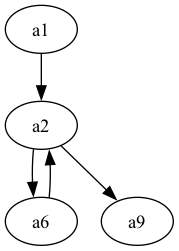
\includegraphics[width=.4\linewidth]{Imagens/fact-desenv-graph.png}
  \caption{Grafo de fluxo de controle}
  \label{fig:sub1}
\end{subfigure}%
\begin{subfigure}{.5\textwidth}
  \centering
  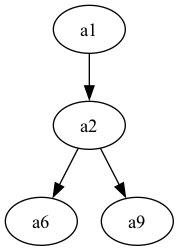
\includegraphics[width=.4\linewidth]{Imagens/fact-desenv-dominance.png}
  \caption{Árvore de dominância}
  \label{fig:sub2}
\end{subfigure}
\caption{CFG e Árvore de Dominância do Código da Figura \ref{fig:exemplo-entrada}}
\label{fig:graph-vs-dom-factorial}
\small{Fonte: O autor}
\end{figure}

A Figura \ref{fig:traducao} apresenta o método de tradução desenvolvido. Sobre a notação utilizada, de mesma forma que as produções gramaticais anotadas com \emph{overline}, funções anotadas com \emph{overline} querem dizer que aquela função é aplicada ponto a ponto. 

A tradução começa por $\mathcal{F}$, que recebe toda a função em SSA e irá retornar a função em ANF, os argumentos são os mesmos da função em SSA. Em termos, a função traduzida contém a tradução do primeiro bloco e a chamada para a função traduzida desse primeiro bloco. Por isso, após em $\mathcal{F}$, $\mathcal{F}_b$ é chamada e faz a tradução do bloco inicial, a qual estarão aninhadas, direta ou indiretamente, todas as demais funções, uma vez que o bloco inicial domina todos os demais. A chamada de cauda da função inicial é a chamada de cauda para função correspondente ao bloco inicial e é o ponto inicial da execução.

A tradução dos blocos em $\mathcal{F}_b$, de mesma forma, é feita retornando uma função em ANF. Os argumentos são determinados pelos $\phi$s do bloco em SSA ($\mathcal{F}_\phi$). Um argumento é gerado para cada $\phi$, e o nome deste argumento é o nome da variável ao qual o resultado da instrução \verb|phi| é atribuído. Após os $\phi$s, o bloco em SSA contém uma lista de definições de variáveis, as quais são traduzidas em $\mathcal{F}_s$. No escopo do bloco sendo traduzido são aninhadas as funções referentes aos blocos dominados imediatamente por este, por isto chama-se recursivamente $\mathcal{F}_b$ para os blocos filhos do bloco sendo traduzido. Toda função em ANF terá uma chamada de cauda, e as chamadas em ANF são traduzidas a partir do \emph{jump} da forma SSA. Se o \emph{jump} da LLVM-IR é o retorno de um valor, esse valor é retornado na função; se esse \emph{jump} é um \emph{branch} sem condicional para outro bloco, a função traduzida referente a este outro bloco é chamada; se há um \emph{branch} condicional na forma SSA, esse \emph{branch} é traduzido para uma condicional na forma ANF.

\begin{figure}[H]
    \begin{tabular}{ l }
    \textbf{Função de Tradução} \\
    $\mathcal{F}(\textbf{define}$ \ $t$ \ $x$ \ $\boldsymbol{(}$ \ $\overline{t \ x}$ \ $\boldsymbol{)}$ \ \textbf{\{} $\overline{b}$ $\textbf{\}})$ \ = \\
    \qquad \textbf{def} \ $x$ \ $\boldsymbol{=}$ \ $\boldsymbol{\lambda}$ $\overline{x}$ \textbf{.let} \ $\overline{\mathcal{F}_b(b)}$ \ \textbf{in} \ $\mathcal{F}_i(b)$ \\
    \qquad onde $b$ = nó inicial de $\overline{b}$ \\ \\
    \textbf{Tradução de um Bloco Básico} \\
    $\mathcal{F}_b(x$ \ \textbf{:} \ $\overline{\phi}$ \ $\overline{s}$ \ $f)$ \ = \\
    \qquad $x$ \ $\boldsymbol{=}$ \ $\boldsymbol{\lambda}$ $\overline{\mathcal{F}_\phi(\phi)}$ \textbf{.let} \ $\overline{\mathcal{F}_s(s)}$ \ $\overline{\mathcal{F}_b(b^\prime)}$ \ \textbf{in} \ $\mathcal{F}_f(x, f)$ \\
    \qquad onde $\overline{b'}$ = nós filhos de $x$ na árvore de dominância \\ \\
    \textbf{Tradução das Declarações} \\
    $\mathcal{F}_s(x \ \boldsymbol{=} \ \beta$ \ $t$ \ $v_1$ \ \textbf{,} \ $v_2)$ \ = \ $x$ \ $\boldsymbol{=}$ \ $v_1$ \ \`{}$\beta$\`{} \  $v_2$ \\
    $\mathcal{F}_s(x \ \boldsymbol{=} \ \mathbf{icmp}$ \ $\tau$ \ $t$ \ $v_1$ \ \textbf{,} \ $v_2)$ \ = \ $x$ \ $\boldsymbol{=}$ \ \textbf{if} \ $v_1$ \ $\tau$ \ $v_2$ \ \textbf{then \ 1 \ else \ 0} \\
    $\mathcal{F}_s(x \ \boldsymbol{=} \ \textbf{select}$ \ $t_c$ \ $v_c$ \ \textbf{,} \ $t_1$ \ $v_1$ \ \textbf{,} \ $t_2$ \ $v_2)$ \ = \ $x$ \ $\boldsymbol{=}$ \ \textbf{if} \ $v_c$ \textbf{/= \ 0 \ then} \ $v_1$ \ \textbf{else} \ $v_2$ \\
    $\mathcal{F}_s(x$ \ $\boldsymbol{=}$ \ $\mu$ \ $t_1$ \ $v$ \ \textbf{to} \ $t_2)$ \ = \ $x$ \ \textbf{=} \ $v$ \\
    $\mathcal{F}_s(x_1$ \ $\boldsymbol{=}$ \ \textbf{call} \ $t$ \ $x_2$ \ $\textbf{(} \ \overline{t \ v} \ \textbf{)})$ \ = \ $x_1$ \ $\boldsymbol{=}$ \ $x_2$ \ $\overline{v}$ \\
    onde $\beta$ e $\tau$ são traduzidos segundo a Tabela \ref{tab:traducao-operacoes} \\ \\
    \textbf{Tradução de um Jump} \\
    $\mathcal{F}_f(x_1$, $\textbf{br}$ \ $t$ \ $x_2)$ \ = \\
    \qquad $x_2$ \ $\overline{\mathcal{F}_p(x_1, \phi)}$ \\
    \qquad onde $x_2$ \ \textbf{:} \ $\overline{\phi}$ \ $\overline{s}$ \ $f$ = bloco com label $x_2$ \\ \\
    $\mathcal{F}_f(x_1$, \textbf{br} \ $t$ \ $v$ \ \textbf{,} \ $t$ \ $x_2$ \ \textbf{,} \ $t$ \ $x_3)$ \ = \\
    \qquad \textbf{if} \ $v$ \ \textbf{$\boldsymbol{\neq}$ \ 0 \ then} \ $x_2$ \ $\overline{\mathcal{F}_p(x_1, \phi_2)}$ \ \textbf{else} \ $x_3$ \ $\overline{\mathcal{F}_p(x_1, \phi_3)}$ \\
    \qquad onde $x_2$ \ \textbf{:} \ $\overline{\phi_2}$ \ $\overline{s_2}$ \ $f_2$ = bloco com label $x_2$ \\
    \enspace \quad \qquad e $x_3$ \ \textbf{:} \ $\overline{\phi_3}$ \ $\overline{s_3}$ \ $f_3$ = bloco com label $x_3$ \\ \\
    $\mathcal{F}_f(x_1$, \textbf{ret} \ $t$ \ $v)$ \ = \ $v$ \\ \\
    \textbf{Encontra os Argumentos de uma Chamada no $\phi$ do Bloco Alvo} \\
    $\mathcal{F}_p(x_1$, $x_2$ \ $\boldsymbol{=}$ \ $\textbf{phi}$ \ $t$ \ $\overline{a})$ \ = \\
    \qquad $v$ \\
    \qquad onde $\textbf{[}$ \ $v$ \ \textbf{,} \ $x_1$ \ \textbf{]} é um elemento de $\overline{a}$ \\ \\
    \textbf{Retorna a Variável Correspondente ao $\phi$} \\
    $\mathcal{F}_\phi(x$ \ $\boldsymbol{=}$ \ $\textbf{phi}$ \ $t$ \ $\overline{a})$ \ = \ $x$ \\ \\
    \textbf{Retorna o \emph{Label} do Bloco} \\
    $\mathcal{F}_i(x$ \ \textbf{:} \ $\overline{\phi}$ \ $\overline{s}$ \ $f)$ \ = \ $x$ \\
    \end{tabular}
    \begin{center}
    \caption{Procedimento de Tradução}
    \label{fig:traducao}
    \small{Fonte: O autor}
    \end{center}
\end{figure}

Em $\mathcal{F}_j$, os argumentos para as chamadas de cauda das funções traduzidas são buscados nos $\phi$s do bloco destino com base no \emph{label} do bloco origem. Por exemplo, se o bloco de \emph{label} $a$ tem um \emph{jump} para o bloco de \emph{label} $b$, e $\overline{\phi}_b$ é o conjunto de $\phi$s de $b$. Então, para cada $\phi_b$ é buscado o argumento $\textbf{[} \ v \ \textbf{,} \ \ l \ \textbf{]}$ onde $l = b$, retornando que o valor do argumento daquela variável na chamada de cauda será $v$.

A Tabela \ref{tab:traducao-operacoes} apresenta o mapeamento das operações nativas da LLVM para expressões equivalentes em Haskell. Tal mapeamento foi feito com base no funcionamento de cada operação, consultando a referência da linguagem da LLVM\footnote{https://llvm.org/docs/LangRef.html}. Primeiramente, nota-se que existem operações da LLVM que se distinguem quanto ao tipo do operando, como: \verb|sdiv| e \verb|udiv|, divisão com sinal (\emph{signed}) e sem sinal (\emph{unsigned}). Essa diferenciação não existe em Haskell, uma vez que foi utilizado somente o tipo Int, portanto esses casos foram mapeados para uma mesma expressão. Além disso, a LLVM possui operações de conversão entre tipos, em Haskell não há a necessidade dessa conversão. As operações bit a bit, como \verb|and|, \verb|or|, \verb|xor|, não são definidas no Prelude de Haskell, portanto foi necessário sempre adicionar uma importação a biblioteca \verb|Data.Bits| no começo dos arquivos Haskell.

Dado um programa bem formatado em SSA, $\mathcal{F}$ retorna um programa bem formatado em ANF. Isso é garantido, uma vez que todas as funções presentes na Figura \ref{fig:traducao} recebem uma produção de uma classe gramatical de entrada, e retornam uma produção de uma das classes gramaticais de saída.

\begin{figure}[h]
\begin{center}
\renewcommand{\ttdefault}{pcr}
\lstset{%
    basicstyle=\ttfamily,
    xleftmargin=.17\textwidth,
    literate={λ}{{$\lambda$}}1 {≠}{{$\neq$}}1,
    emph={def, =, ., let, in, if, else, then},
    emphstyle={\bfseries},
}
\begin{lstlisting}[mathescape]
def factorial $\boldsymbol=$
    $\boldsymbol{\lambda}$a0.let
        a1 $\boldsymbol=$ $\boldsymbol{\lambda.}$let
            a2 $\boldsymbol=$ $\boldsymbol{\lambda}$a3 a4.let
                a5 $\boldsymbol=$ if a4 < 2 then $\mathbf{1}$ else $\mathbf{0}$
                a6 $\boldsymbol=$ $\boldsymbol{\lambda.}$let
                         a7 $\boldsymbol=$ a4 + (-1)
                         a8 $\boldsymbol=$ a3 * a4
                     in a2 a8 a7
                a9 $\boldsymbol=$ $\boldsymbol{\lambda}$.let
                         a10 $\boldsymbol=$ a3 * i
                     in a10
            in if a5 $\boldsymbol{\neq}$ $\textbf{0}$ then a9
                          else a6
        in a2 1 a0
    in a1
\end{lstlisting}
\caption{ANF de Saída de $\mathcal{F}$ a partir do Código da Figura \ref{fig:exemplo-entrada}}
\label{fig:exemplo-saida}
\small{Fonte: O autor, saída do tradutor desenvolvido}
\end{center}
\end{figure}

Um exemplo de resultado desta tradução para o código da Figura \ref{fig:exemplo-entrada} pode ser visto na Figura \ref{fig:exemplo-saida}. Neste exemplo o código segue exatamente a gramática aqui descrita, porém, conforme comentado, essa notação é diferente, mas diretamente correspondente a como a saída do tradutor é dada. Na prática o código resultante da tradução implementada é código Haskell compilável no GHC. A Figura \ref{fig:exemplo-saida-haskell} apresenta um exemplo de como é o resultado exato dado pelo tradutor para essa mesma entrada (código da Figura \ref{fig:exemplo-entrada}), na qual nota-se que a diferença é apenas quanto ao padrão da notação.

Algo importante de abordar nesse ponto é quanto ao tratamento das variáveis, já que as regras para definição de  identificadores de variáveis da LLVM-IR não são compatíveis com as do Haskell. Como visto nos exemplos, em LLVM-IR, as variáveis locais começam com "\verb|%|"\ e podem ser qualquer sequência de caracteres, inclusive começando com números, o que não é permitido em Haskell. Portanto, para obter código válido em Haskell, um dos tratamentos feitos foi remover o "\verb|%|"\ no inicio das variáveis locais substituindo por um caractere "\verb|a|".

Ademais, há um detalhe quanto a expressão de ANF em Haskell, pois conforme citado, ANF adota avaliação \emph{call-by-value} \cite{flanagan1993essence}, enquanto que a avaliação em Haskell é \emph{call-by-need}. Portanto, para que o código gerado tenha o mesmo comportamento sob ambas semânticas, em algumas definições é adicionado um parâmetro unit "()", assim transformando tais expressões em declarações de funções e garantido que não seriam avaliadas no momento de sua definição mesmo em uma linguagem cuja ordem de avaliação seja \emph{call-by-value}. Além disso esse parâmetro é necessário para manter que a sintaxe de ANF seja mantida e não permita expressões \emph{let} aninhadas \cite{sabry1992reasoning}. Esse é um parâmetro que não irá ser usado dentro das funções, por isso foi escolhido o tipo \emph{Unit} "()" do Haskell.

\begin{table}[h]
    \begin{center}
    \begin{tabular}{ l | l }
    \textbf{LLVM-IR} & \textbf{Haskell} \\
    \hline \hline
    \multicolumn{2}{ c }{\textbf{Operações Binárias}} \\
    \hline
        $x$\ \textbf{=}\ \textbf{add} \ $t$ \ $v_1$ \ \textbf{,} \ $v_2$ & $x$ \ \textbf{=} $v_1$ \textbf{+} \ $v_2$ \\
    \hline
    $x$\ \textbf{=}\ \textbf{sub} \ $t$ \ $v_1$ \ \textbf{,} \ $v_2$ & $x$ \ \textbf{=} $v_1$ \textbf{-} \ $v_2$ \\
    \hline
    $x$\ \textbf{=}\ \textbf{mul} \ $t$ \ $v_1$ \ \textbf{,} \ $v_2$ & $x$ \ \textbf{=} $v_1$ \textbf{*} \ $v_2$ \\
    \hline
    $x$\ \textbf{=}\ \textbf{udiv} \ $t$ \ $v_1$ \ \textbf{,} \ $v_2$ & $x$ \ \textbf{=} $v_1$ \textbf{`div`} \ $v_2$ \\
    \hline
    $x$\ \textbf{=}\ \textbf{sdiv} \ $t$ \ $v_1$ \ \textbf{,} \ $v_2$ & $x$ \ \textbf{=} $v_1$ \textbf{`div`} \ $v_2$ \\
    \hline
    $x$\ \textbf{=}\ \textbf{urem} \ $t$ \ $v_1$ \ \textbf{,} \ $v_2$ & $x$ \ \textbf{=} $v_1$ \textbf{`mod`} \ $v_2$ \\
    \hline
    $x$\ \textbf{=}\ \textbf{srem} \ $t$ \ $v_1$ \ \textbf{,} \ $v_2$ & $x$ \ \textbf{=} $v_1$ \textbf{`mod`} \ $v_2$ \\
    \hline
    $x$\ \textbf{=}\ \textbf{and} \ $t$ \ $v_1$ \ \textbf{,} \ $v_2$ & $x$ \ \textbf{=} $v_1$ \textbf{ $.\&.$ } \ $v_2$ \\
    \hline
    $x$\ \textbf{=}\ \textbf{or} \ $t$ \ $v_1$ \ \textbf{,} \ $v_2$ & $x$ \ \textbf{=} $v_1$ \textbf{ $.|.$ } \ $v_2$ \\
    \hline
    $x$\ \textbf{=}\ \textbf{xor} \ $t$ \ $v_1$ \ \textbf{,} \ $v_2$ & $x$ \ \textbf{=} $v_1$ \textbf{ `xor` } \ $v_2$ \\
    \hline
    $x$\ \textbf{=}\ \textbf{shl} \ $t$ \ $v_1$ \ \textbf{,} \ $v_2$ & $x$ \ \textbf{=} $v_1$ \textbf{ `shiftL` } \ $v_2$ \\
    \hline
    $x$\ \textbf{=}\ \textbf{lshr} \ $t$ \ $v_1$ \ \textbf{,} \ $v_2$ & $x$ \ \textbf{=} $v_1$ \textbf{ `shiftR` } \ $v_2$ \\
    \hline
    \multicolumn{2}{ c }{\textbf{Operações de Comparação}} \\
    \hline
    $x$\ \textbf{=}\ \textbf{icmp} \ \textbf{eq} \ $t$ \ $v_1$ \ \textbf{,} \ $v_2$ & $x$ \ \textbf{=} \ \textbf{if} \ $v_1$ \ \textbf{==} \ $v_2$ \ \textbf{then \ 1 \ else \ 0}\\
    \hline
    $x$\ \textbf{=}\ \textbf{icmp} \ \textbf{ne} \ $t$ \ $v_1$ \ \textbf{,} \ $v_2$ & $x$ \ \textbf{=} \ \textbf{if} \ $v_1$ \ \textbf{/=} \ $v_2$ \ \textbf{then \ 1 \ else \ 0}\\
    \hline
    $x$\ \textbf{=}\ \textbf{icmp} \ \textbf{ugt} \ $t$ \ $v_1$ \ \textbf{,} \ $v_2$ & $x$ \ \textbf{=} \ \textbf{if} \ $v_1$ \ \textbf{>} \ $v_2$ \ \textbf{then \ 1 \ else \ 0}\\
    \hline
    $x$\ \textbf{=}\ \textbf{icmp} \ \textbf{uge} \ $t$ \ $v_1$ \ \textbf{,} \ $v_2$ & $x$ \ \textbf{=} \ \textbf{if} \ $v_1$ \ \textbf{>=} \ $v_2$ \ \textbf{then \ 1 \ else \ 0}\\
    \hline
    $x$\ \textbf{=}\ \textbf{icmp} \ \textbf{ult} \ $t$ \ $v_1$ \ \textbf{,} \ $v_2$ & $x$ \ \textbf{=} \ \textbf{if} \ $v_1$ \ \textbf{<} \ $v_2$ \ \textbf{then \ 1 \ else \ 0}\\
    \hline
    $x$\ \textbf{=}\ \textbf{icmp} \ \textbf{ule} \ $t$ \ $v_1$ \ \textbf{,} \ $v_2$ & $x$ \ \textbf{=} \ \textbf{if} \ $v_1$ \ \textbf{<=} \ $v_2$ \ \textbf{then \ 1 \ else \ 0}\\
    \hline
    $x$\ \textbf{=}\ \textbf{icmp} \ \textbf{sgt} \ $t$ \ $v_1$ \ \textbf{,} \ $v_2$ & $x$ \ \textbf{=} \ \textbf{if} \ $v_1$ \ \textbf{>} \ $v_2$ \ \textbf{then \ 1 \ else \ 0}\\
    \hline
    $x$\ \textbf{=}\ \textbf{icmp} \ \textbf{sge} \ $t$ \ $v_1$ \ \textbf{,} \ $v_2$ & $x$ \ \textbf{=} \ \textbf{if} \ $v_1$ \ \textbf{>=} \ $v_2$ \ \textbf{then \ 1 \ else \ 0}\\
    \hline
    $x$\ \textbf{=}\ \textbf{icmp} \ \textbf{slt} \ $t$ \ $v_1$ \ \textbf{,} \ $v_2$ & $x$ \ \textbf{=} \ \textbf{if} \ $v_1$ \ \textbf{<} \ $v_2$ \ \textbf{then \ 1 \ else \ 0}\\
    \hline
    $x$\ \textbf{=}\ \textbf{icmp} \ \textbf{sle} \ $t$ \ $v_1$ \ \textbf{,} \ $v_2$ & $x$ \ \textbf{=} \ \textbf{if} \ $v_1$ \ \textbf{<=} \ $v_2$ \ \textbf{then \ 1 \ else \ 0}\\
    \hline
    \multicolumn{2}{ c }{\textbf{Operação de Seleção}} \\
    \hline
    $x$ \ \textbf{=} \ \textbf{select} \ $t_1$ \ $v_1$ \ \textbf{,} \ $t_2$ \ $v_2$ \textbf{,} \ $t_3$ \ $v_3$ & $x$ \ \textbf{=} \ \textbf{if} \ $v_1$ \textbf{== \ 1 \ then} \ $v_2$ \ \textbf{else} \ $v_3$ \\
    \hline
    \multicolumn{2}{ c }{\textbf{Operações de Conversão}} \\
    \hline
    $x$ \ \textbf{=} \ $\mu$ \ $t_1$ \ $v$ \ \textbf{to} \ $t_2$ & $x$ \ \textbf{=} \ $v$ \\
    \hline
    \multicolumn{2}{ c }{\textbf{Chamada de Função}} \\
    \hline
    $x$ \ \textbf{=} \ \textbf{call} \ $t_1$ \ $x_f$ \ \textbf{(} \ $\overline{y}$ \ \textbf{)} & $x$ \ \textbf{=} \ $x_f$ \ $\overline{y}$ \\
    \hline
    \end{tabular}
    \caption{Tradução das Operações Nativas da LLVM}
    \label{tab:traducao-operacoes}
    \small{Fonte: O autor}
    \end{center}
\end{table}

\begin{figure}[h]
\centering
\lstset{xleftmargin=.24\textwidth}
\begin{lstlisting}[language=haskell,style=nasm]
import Data.Bits

factorial a0 =
  let
    a1 () =
      let
        a2 a3 a4 =
          let
            a5 = if a4 < 2 then 1 else 0
            a6 () =
              let
                a7 = a4 + (-1)
                a8 = a3 * a4
              in a2 a8 a7
            a9 () =
              let
                a10 = a3 * 1
              in a10 
          in if a5 /= 0
            then a9 ()
            else a6 ()
      in a2 1 a0
  in a1 ()
\end{lstlisting}
\caption{Tradução Resultante para o Exemplo da Figura \ref{fig:exemplo-entrada}}
\label{fig:exemplo-saida-haskell}
\small{Fonte: O autor, resultado dado pelo tradutor implementado}
\end{figure}

\section{Resultados}

Nesta seção a tradução implementada é aplicada a mais exemplos, e os resultados são extraídos e discutidos. Os exemplos apresentados são as traduções de: um código de divisão segura, o Algoritmo de Euclides para o calculo do Máximo Divisor Comum \cite{knuth2014art}, e um algoritmo \emph{naïve} de checagem de primos. Os códigos de exemplo em LLVM-IR foram gerados a partir de código C, usando o \emph{clang} versão \verb|15.0.0| em uma máquina com processador \verb|Apple M1 Pro|, e foi utilizado com o seguinte comando:

\begin{verbatim}
clang -S -emit-llvm -O1 -g0 <arquivo.c> -o <arquivo.ll>
\end{verbatim}

Os códigos gerados foram editados com três objetivos: remover palavras chaves que são ignoradas na análise léxica; a adição explicitamente do \emph{label} ao primeiro bloco, uma vez que esta não é gerada automaticamente pelo \emph{clang}; as funções são traduzidas com alterações em seu nome, foi colocado novamente o nome segundo da função do código de entrada. Para que não fuja ao escopo deste trabalho, nesses exemplos são utilizados somente tipos inteiros simples: sem ponteiros, \emph{arrays} ou tipos compostos. Além dos exemplos expostos nesta seção, o repositório deste trabalho\footnote{https://github.com/IgorFroehner/llvm-ssa-to-functional} conta com outros exemplos como: soma de inteiros até $n$, exponenciação modular, busca binária da raiz quadrada de um inteiro, e cálculo da função totiente de Euler.

\subsection{Divisão Segura}

Nesse exemplo foi criada uma função em C++ que recebe dois inteiros, em que $n$ é o dividendo e $d$ é o divisor, retornando -1 se $d = 0$, se não retorna o resultado da divisão inteira de $n$ por $d$.

\begin{figure}[ht]
    \centering
    \begin{subfigure}[b]{\textwidth}
        \centering
        \lstset{xleftmargin=.3\textwidth}
        \begin{lstlisting}[language=c,style=nasm]
int safe_div(int n, int d) {
    if (d == 0) return -1;
    else return n / d;
}
        \end{lstlisting}
        \caption{Divisão Segura em C++}
        \label{fig:image1}
    \end{subfigure}

    \vspace{1em} % Adds vertical space between the images

    \begin{subfigure}[b]{\textwidth}
        \begin{center}
        \lstset{xleftmargin=.24\textwidth}
        \begin{lstlisting}[language=llvm,style=nasm]
define i32 @safe_div(i32 %0, i32 %1) {
2:
  %3 = icmp eq i32 %1, 0
  br i1 %3, label %6, label %4

4:
  %5 = sdiv i32 %0, %1
  br label %6

6:
  %7 = phi i32 [ %5, %4 ], [ -1, %2 ]
  ret i32 %7
}
        \end{lstlisting}
        \caption{Divisão Segura em LLVM-IR}
        \label{fig:safe-div-llvm}
        \end{center}
    \end{subfigure}

    \vspace{.5em} % Adds vertical space between the images
    
    \caption{Exemplo de Código Fonte de Divisão Segura}
    \label{fig:safe-div}
    \small{Fonte: O autor, gerado usando \emph{clang} e editado}
\end{figure}

Constata-se no código na Figura \ref{fig:safe-div-llvm} e também no CFG e árvore de dominância na Figura \ref{fig:graph-vs-dom-safe-div}, que este é um exemplo simples que contém somente três blocos. O primeiro bloco usa uma instrução \verb|icmp| para fazer a comparação do segundo argumento com $0$. A variável \verb|%3|, é definida com o valor $1$ se \verb|%1| é igual (\verb|eq|) a zero, se não recebe $0$. A instrução \verb|br| checa se o valor em \verb|%3| é verdadeiro ($\neq 0$), e em caso positivo direcionando o fluxo para o bloco de \emph{label} \verb|6|, em caso negativo é dirigido ao bloco de \emph{label} \verb|4|. No bloco \verb|4| a divisão com sinal é feita e a execução vai para o bloco \verb|6|. O bloco 6 faz o retorno do resultado, em que, pela instrução \verb|phi| depende de se o fluxo veio a partir do bloco \verb|2|, ou \verb|4|.

\begin{figure}[H]
\centering
\begin{subfigure}{.5\textwidth}
  \centering
  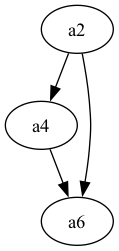
\includegraphics[width=.2\linewidth]{Imagens/safe_div_graph.png}
  \caption{Grafo de fluxo de controle}
  \label{fig:sub1}
\end{subfigure}%
\begin{subfigure}{.5\textwidth}
  \centering
  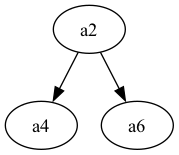
\includegraphics[width=.4\linewidth]{Imagens/safe_div_dominance.png}
  \caption{Árvore de dominância}
  \label{fig:sub2}
\end{subfigure}
\caption{CFG e Árvore de Dominância do Código de Divisão Segura}
\label{fig:graph-vs-dom-safe-div}
\small{Fonte: O autor}
\end{figure}

\begin{figure}[H]
\centering
\lstset{xleftmargin=.25\textwidth}
\begin{lstlisting}[language=haskell,style=nasm]
import Data.Bits

safe_div a0 a1 =
  let
    a2 () =
      let
        a3 = if a1 == 0 then 1 else 0
        a4 () =
          let
            a5 = a0 `div` a1
          in a6 a5
        a6 a7 =
          let
          in a7 
      in if a3 /= 0
        then a6 (-1)
        else a4 ()
  in a2 ()
\end{lstlisting}
\caption{Tradução Resultante do Exemplo de Divisão Segura}
\label{fig:safe-div-saida}
\small{Fonte: O autor, resultado dado pelo tradutor implementado}
\end{figure}

A Figura \ref{fig:safe-div-saida} contém o resultado da saída do tradutor implementado. Esse resultado é código Haskell e pode ser carregado no GHC e executado. Nota-se que na tradução as funções são equivalentes aos blocos da forma SSA: \verb|a2|, \verb|a4|, \verb|a6|. Com as funções \verb|a4| e \verb|a6| aninhadas a função \verb|a2|, visto que o bloco de \emph{label} \verb|2| domina imediatamente os outros blocos. Nota-se também que a função \verb|a6| tem um argumento, que corresponde a instrução \verb|phi| atribuída a \verb|%7|. Nas suas chamadas de cauda, \verb|a2| chama condicionalmente \verb|a6| com valor $-1$, e \verb|a4| usa como argumento a variável \verb|a5|.

\subsection{Algoritmo de Euclides}

Sendo $u$ e $v$ inteiros não nulos, o Maior Divisor Comum (GCD, do inglês \emph{Greatest Common Divisor}) é o maior inteiro que divide $u$ e $v$ sem deixar resto \cite{knuth2014art}. No Livro 7 de "Elementos" \ de Euclides, um algoritmo para calcular o GCD é descrito, que veio a ser conhecido como Algoritmo de Euclides. A Figura \ref{fig:euclides-cpp} apresenta uma implementação recursiva desse algoritmo na linguagem C, e esse código foi utilizado para gerar o exemplo de entrada em LLVM-IR da Figura \ref{fig:euclides-llvm}.

Este exemplo contém quatro blocos básicos: o bloco \verb|2| somente leva a execução ao bloco \verb|3|, no bloco \verb|3| há duas instruções \verb|phi| a comparação e um \emph{branch} que usa o valor da comparação, o bloco \verb|7| calcula o resto (\verb|srem|) e volta para o bloco \verb|3|, e por fim o bloco \verb|9| que somente faz o retorno do resultado armazenado na variável \verb|%4|. Neste exemplo há um um \emph{loop} entre os blocos \verb|a3| e \verb|a7|, que fica evidenciado no CFG na Figura \ref{fig:graph-vs-dom-gcd}, e que fica também explícito após a tradução nas chamadas de cauda das funções.

\begin{figure}[H]
    \centering
    \begin{subfigure}[b]{\textwidth}
        \centering
        \lstset{xleftmargin=.22\textwidth}
        \begin{lstlisting}[language=c,style=nasm]
int euclides_gcd(int a, int b) {
    if (b == 0) return a;
    else return euclides_gcd(b, a % b);
}
        \end{lstlisting}
        \caption{Algoritmo de Euclides em C}
        \label{fig:euclides-cpp}
    \end{subfigure}

    \vspace{1em} % Adds vertical space between the images

    \begin{subfigure}[b]{\textwidth}
        \begin{center}
        \lstset{xleftmargin=.20\textwidth}
        \begin{lstlisting}[language=llvm,style=nasm]
define i32 @euclides_gcd(i32 %0, i32 %1) {
2:
  br label %3

3:
  %4 = phi i32 [ %0, %2 ], [ %5, %7 ]
  %5 = phi i32 [ %1, %2 ], [ %8, %7 ]
  %6 = icmp eq i32 %5, 0
  br i1 %6, label %9, label %7

7:
  %8 = srem i32 %4, %5
  br label %3

9:
  ret i32 %4
}
        \end{lstlisting}
        \caption{Algoritmo de Euclides em LLVM-IR}
        \label{fig:euclides-llvm}
        \end{center}
    \end{subfigure}

    \vspace{.5em} % Adds vertical space between the images
    
    \caption{Algoritmo de Euclides em LLVM-IR}
    \label{fig:euclides-entrada}
    \small{Fonte: O autor, gerado usando \emph{clang} e editado}
\end{figure}

Segue do exemplo do Algoritmo de Euclides a tradução apresentada na Figura \ref{fig:euclides-saida}, com as quatro funções que correspondem aos quatro blocos da forma SSA. Destaca-se que a função \verb|a9| apenas retorna o valor recebido como argumento, assim como na forma SSA. As instruções \verb|phi| do bloco \verb|3| são traduzidos para os dois parâmetros da função \verb|a3|, e o valor que essa variável assume é definido dependendo de qual função está fazendo a chamada.

\begin{figure}[H]
\centering
\begin{subfigure}{.5\textwidth}
  \centering
  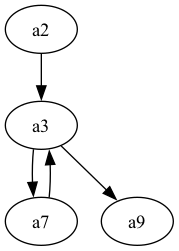
\includegraphics[width=.4\linewidth]{Imagens/gcd_graph.png}
  \caption{Grafo de fluxo de controle}
  \label{fig:sub1}
\end{subfigure}%
\begin{subfigure}{.5\textwidth}
  \centering
  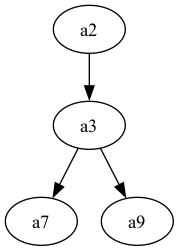
\includegraphics[width=.4\linewidth]{Imagens/gcd_dominance.png}
  \caption{Árvore de dominância}
  \label{fig:sub2}
\end{subfigure}
\caption{CFG e Árvore de Dominância do Código do Algoritmo de Euclides}
\label{fig:graph-vs-dom-gcd}
\small{Fonte: O autor}
\end{figure}

\begin{figure}[H]
\centering
\lstset{xleftmargin=.23\textwidth}
\begin{lstlisting}[language=haskell,style=nasm]
import Data.Bits

euclides_gcd a0 a1 =
  let
    a2 () =
      let
        a3 a4 a5 =
          let
            a6 = if a5 == 0 then 1 else 0
            a7 () =
              let
                a8 = a4 `mod` a5
              in a3 a5 a8
            a9 () =
              let
              in a4 
          in if a6 /= 0
            then a9 ()
            else a7 ()
      in a3 a0 a1
  in a2 ()
\end{lstlisting}
\caption{Tradução Resultante para o Exemplo do Algoritmo de Euclides}
\label{fig:euclides-saida}
\small{Fonte: O autor, resultado dado pelo tradutor implementado}
\end{figure}

\subsection{Teste de Primalidade}

Para obter um exemplo maior, foi utilizado um algoritmo \emph{naïve} de checagem de primalidade. O código da Figura \ref{fig:primo-c} recebe um inteiro \verb|num|, e se \verb|num <= 1| retorna \verb|0|, se não, faz um laço com \verb|i|, de dois até raiz quadrada de \verb|num| com passo um. E dentro da execução do laço, se \verb|num| é divisível por \verb|i| então \verb|num| não é primo. Se o laço de repetição termina sem retornar, então \verb|num| é primo.

\begin{figure}[h]
    \centering
    \begin{subfigure}[b]{\textwidth}
        \centering
        \lstset{xleftmargin=.2\textwidth}
        \begin{lstlisting}[language=c,style=nasm]
int is_prime(int num) {
    if (num <= 1) return 0;
    for (int i = 2; i * i <= num; i++) {
        if (num % i == 0) return 0;
    }
    return 1;
}
        \end{lstlisting}
        \caption{Teste de Primalidade \emph{Naïve} em C}
        \label{fig:primo-c}
    \end{subfigure}

    \vspace{1em} % Adds vertical space between the images

    \begin{subfigure}[b]{\textwidth}
        \begin{center}
        \lstset{xleftmargin=.21\textwidth}
        \begin{lstlisting}[language=llvm,style=nasm]
define i32 @is_prime(i32 %0) {
1:
  %2 = icmp slt i32 %0, 2
  br i1 %2, label %19, label %3

3:
  %4 = icmp slt i32 %0, 4
  %5 = and i32 %0, 1
  %6 = icmp eq i32 %5, 0
  %7 = or i1 %4, %6
  br i1 %7, label %16, label %8

8:
  %9 = phi i32 [ %10, %13 ], [ 2, %3 ]
  %10 = add nuw nsw i32 %9, 1
  %11 = mul nsw i32 %10, %10
  %12 = icmp sgt i32 %11, %0
  br i1 %12, label %16, label %13

13:
  %14 = srem i32 %0, %10
  %15 = icmp eq i32 %14, 0
  br i1 %15, label %16, label %8

16:
  %17 = phi i1 [ %4, %3 ], [ %12, %8 ], [ %12, %13 ]
  %18 = zext i1 %17 to i32
  br label %19

19:
  %20 = phi i32 [ 0, %1 ], [ %18, %16 ]
  ret i32 %20
}
        \end{lstlisting}
        \caption{Teste de Primalidade \emph{Naïve} em LLVM-IR}
        \end{center}
    \end{subfigure}

    \vspace{.5em} % Adds vertical space between the images
    
    \caption{Exemplo de Teste de Primalidade}
    \label{fig:primo-entrada}
    \small{Fonte: O autor, gerado usando \emph{clang} e editado}
\end{figure}

O código em LLVM-IR gerado a partir desse exemplo contém seis blocos, três dos quais \verb|8|, \verb|16| e \verb|19| tem instruções \verb|phi|. Observa-se que a instrução \verb|phi| atribuída a variável \verb|17| contém três argumentos, que acontece pelo fato de o fluxo chegar ao bloco \verb|16| a partir de outros três blocos e que o valor de \verb|17| é determinado pelo bloco que levou a execução até o \verb|16|. Nota-se na Figura \ref{fig:graph-vs-dom-prime} que esse exemplo contém um grafo de fluxo de controle mais notável, em que a árvore de dominância desempenha um papel importante ao apontar os escopos das variáveis e das funções após para a tradução.

Segue da aplicação da tradução nesse exemplo o resultado visto na Figura \ref{fig:primo-saida}. Código que contém seis funções, e pode-se perceber que as funções \verb|a8|, \verb|a16| e \verb|a19| têm suas instruções \verb|phi| traduzidas para seus argumentos. Pontua-se também que a variável \verb|%17|, que na forma SSA é atribuída à instrução \verb|phi| com três argumentos, e no código traduzido há três chamadas para a função \verb|a16|. Além disso, neste exemplo são usados operadores bit a bit, o "ou" \ (.|.) e o "e" \ (.\&.), que são definidos na biblioteca \verb|Data.Bits|.

Para comentar mais como a árvore de dominância é utilizada para definir o escopo das funções, pela Figura \ref{fig:graph-vs-dom-prime}, observa-se que o bloco \verb|a8| domina imediatamente somente o bloco \verb|a13|. Fazendo com que a função traduzida \verb|a13| exista somente dentro do escopo da função \verb|a8|.

\begin{figure}[h]
\centering
\lstset{xleftmargin=.16\textwidth}
\begin{lstlisting}[language=haskell,style=nasm]
import Data.Bits

is_prime a0 =
  let
    a1 () =
      let
        a2 = if a0 < 2 then 1 else 0
        a3 () =
          let
            a4 = if a0 < 4 then 1 else 0
            a5 = a0 .&. 1
            a6 = if a5 == 0 then 1 else 0
            a7 = a4 .|. a6
            a8 a9 =
              let
                a10 = a9 + 1
                a11 = a10 * a10
                a12 = if a11 > a0 then 1 else 0
                a13 () =
                  let
                    a14 = a0 `mod` a10
                    a15 = if a14 == 0 then 1 else 0
                  in if a15 /= 0
                    then a16 a12
                    else a8 a10
              in if a12 /= 0
                then a16 a12
                else a13 ()
            a16 a17 =
              let
                a18 = a17
              in a19 a18
          in if a7 /= 0
            then a16 a4
            else a8 2
        a19 a20 =
          let
          in a20 
      in if a2 /= 0
        then a19 0
        else a3 ()
  in a1 ()
\end{lstlisting}
\caption{Tradução Resultante do Exemplo de Teste de Primalidade}
\label{fig:primo-saida}
\small{Fonte: O autor}
\end{figure}

\begin{figure}[h]
\centering
\begin{subfigure}{.5\textwidth}
  \centering
  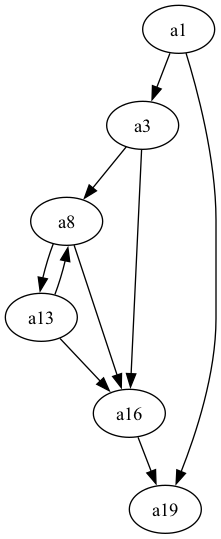
\includegraphics[width=.4\linewidth]{Imagens/prime_graph.png}
  \caption{Grafo de fluxo de controle}
\end{subfigure}%
\begin{subfigure}{.5\textwidth}
  \centering
  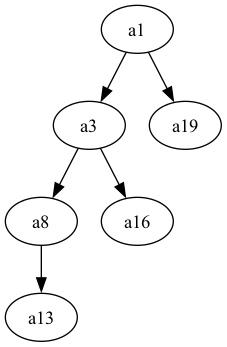
\includegraphics[width=.5\linewidth]{Imagens/prime_dominance.png}
  \caption{Árvore de dominância}
\end{subfigure}
\caption{CFG e Árvore de Dominância do Código de Teste de Primalidade}
\label{fig:graph-vs-dom-prime}
\small{Fonte: O autor}
\end{figure}

\section{Discussão}

Nessa seção será feita uma discussão sobre o que se mostrou possível traduzir através do método proposto. De início é possível comentar que a LLVM é um conjunto de ferramentas de tradução de código capaz de compilar projetos grandes com diversos arquivos, funções e bibliotecas. Porém nesse trabalho são traduzidas somente funções puras em um arquivo, permitindo também somente a chamada para outras funções puras. Além disso, como foi citado, a LLVM-IR conta com diversos tipos nativos e instrumentação robusta para definição de tipos compostos, enquanto que neste trabalho foram tratados somente de tipos inteiros simples.

Em termos: o método implementado nesse trabalho é capaz de traduzir funções puras que usam somente tipos inteiros simples de LLVM-IR para código Haskell em ANF. O fato de apenas funções puras serem traduzidas quer dizer que não foram tratados efeitos colaterais. Por exemplo: não são permitidas variáveis globais mutáveis, são compreendidos somente tipos inteiros simples (restringindo o uso de ponteiros de memória), não foi mapeada nenhuma chamada de sistema operacional, entre outras funcionalidades que fariam o uso de efeitos colaterais.

Desde a interpretação do código de entrada em LLVM-IR, por meio da definição da gramática livre de contexto, é garantida uma parte da pureza das funções. Isso se dá pois a gramática de entrada não permite variáveis globais, não mapeia operações que possam causar efeitos, e todas as instruções nativas da LLVM interpretadas são puras (sem mais efeitos além de receberem valores e retornarem um valor). Porém é importante pontuar que a imutabilidade das variáveis não é checada durante a tradução, mas para que o método possa traduzir corretamente, uma entrada válida em LLVM-IR é exigida.

Para estender a tradução e adicionar o tratamento de efeitos colaterais, pode ser estudado o uso da metalinguagem monádica apresentada por \citeonline{moggi1988computational}. Essa tese se fundamenta no fato de que, apesar de que \citeonline{sabry1992reasoning} estavam interessados em descobrir como aplicar otimizações tradicionais sem utilizar CPS quando introduziram o ANF, eles também demonstram que o cálculo obtido é equivalente ao cálculo-$\lambda$ computacional descrito por \citeonline{moggi1991notions}. Dada essa relação, e sabendo que, dessa forma, o cálculo usado pelo ANF é capaz de representar quaisquer efeitos computacionais, é possível estudar a definição de uma tradução sintática para a metalinguagem monádica de \citeonline{moggi1988computational}, o que permitiria a execução do código contendo efeitos colaterais dentro do GHC/Haskell.


\chapter{Conclusão}\label{cap:conclusao}

Há diversos desafios e problemas a serem superados na área de compiladores. As representações intermediárias têm um papel importante ao permitir algoritmos de otimizações de código eficientes. Uma vez que compiladores têm se voltado cada vez mais para modelos modulares, as representações intermediárias têm sido usadas para promover a integração entre os módulos dos compiladores e a eficiência dos algoritmos de otimização.

A forma SSA favorece diversas otimizações de código quanto ao fluxo de dados e de controle em compiladores de linguagens imperativas. Isso segue dos fatos que SSA tem uma representação em grafo de fluxo de controle, limita que cada variável seja definida somente uma vez e define a notação conceitual da função $\phi$, de forma que o fluxo de dados fica explícito aos algoritmos de otimização. Tendo sua evidência quanto à otimização de programas, SSA é usada para fundamentar a representação intermediária da LLVM, a LLVM-IR.

A LLVM é o \emph{framework} de compilação de código que está no estado da arte atualmente. É utilizada no \emph{clang} para as linguagens C e C++, na construção do compilador do Rust, e encontra aplicações na compilação ou interpretação de linguagens como Java, Python, Ruby, TypeScript, entre outras. A LLVM se destaca por oferecer um \emph{backend} de compilação robusto, oferecendo uma ampla gama de otimizações com uma interface que é ao mesmo tempo acessível e transparente, facilitando o desenvolvimento e a implementação de novos compiladores.

Tendo em vista o fatos de que SSA é correspondente a programação funcional \cite{kelsey1995correspondence} e ANF \cite{ssaToAnf}, e que a LLVM fundamenta sua representação intermediária em SSA, esse trabalho buscou explorar a tradução entre código em LLVM-IR na forma SSA, para ANF em Haskell. Para isso, foi definido um subconjunto da LLVM-IR, e foi desenvolvida uma tradução adaptada do método descrito por \citeonline{ssaToAnf}. 

A partir da pesquisa feita, foi possível estabelecer uma tradução de funções puras com tipos inteiros simples da LLVM-IR para representação funcional em ANF na linguagem Haskell. Portanto, a principal ressalva levantada nesse trabalho é que o tratamento de efeitos colaterais nessa tradução necessita do desenvolvimento de uma extensão do método proposto.

A implementação do método de tradução proposto foi feita na linguagem Haskell, foram utilizadas bibliotecas como Alex\footnote{https://hackage.haskell.org/package/alex} para análise léxica, Happy\footnote{https://hackage.haskell.org/package/happy} para análise sintática e FGL\footnote{https://hackage.haskell.org/package/fgl} (\emph{Functional Graph Library}) para grafos. No programa desenvolvido há opções para gerar representações gráficas do grafo de fluxo de controle e da árvore de dominância, o que pode facilitar o entendimento da saída das traduções. O código implementado está disponível em um repositório aberto no GitHub\footnote{https://github.com/IgorFroehner/llvm-ssa-to-functional}.

\section{Trabalhos Futuros}

Há algumas oportunidades de pesquisas que podem ser exploradas em trabalhos futuros com base no resultado obtido. Um caminho inicial seria aumentar a gama de tipos nativos e instruções da LLVM que são aceitos na interpretação, mas ainda mantendo a característica de tradução limitada a funções puras. O que ajudaria mais à frente a compreender se a tradução proposta é adequada para um subconjunto maior da LLVM-IR, ou como esse método precisaria ser estendido.

Conforme comentado durante a explicação da proposta do trabalho, \citeonline{rigon2020inferring} exploraram a correspondência entre SSA e ANF e puderam inferir tipos e efeitos em uma linguagem pseudo-imperativa. Com o resultado do presente trabalho é possível futuramente investigar a inferência de tipos e efeitos sobre código em LLVM-IR, ou seja, código gerado a partir de linguagens imperativas como C, C++ ou Rust. Ou ainda, quanto ao tratamento de efeitos colaterais, há a possibilidade de estudar o desenvolvimento de uma tradução estática para a metalinguagem monádica de \citeonline{moggi1988computational}.

Além disso, a justificativa do presente trabalho se fundamentou no fato de que as representações intermediárias, ANF e SSA, tornam mais eficazes alguns algoritmos de otimização de código. Outra pesquisa futura possível seria buscar aplicar os códigos de saída deste trabalho a algoritmos de otimização presentes na literatura e validar se benefícios seriam atingidos.


% -----------------------------------------------------------------
% ELEMENTOS PÓS-TEXTUAIS
% -----------------------------------------------------------------
\postextual

% Você pode comentar os elementos que não deseja em seu trabalho;

% Referências bibliográficas
\bibliography{Referencias}	% Elemento Obrigatório

%\include{PosTextuais/Glossario}			% Elemento Opcional
%\include{PosTextuais/Apendices}			% Elemento Opcional
%\include{PosTextuais/Anexos}				% Elemento Opcional
%\include{PosTextuais/IndiceRemissivo}		% Elemento Opcional

\end{document}

% -----------------------------------------------------------------
% Fim do Documento
% -----------------------------------------------------------------	
